% Nexa Drive — project report in ACL format (preprint mode). Compile with XeLaTeX, e.g.
%   conda run -n baocao tectonic report/main.tex
\documentclass[11pt]{article}
\usepackage[preprint]{acl}

\usepackage{fontspec}
% Times-like font that covers Vietnamese diacritics (loaded by file name: Tectonic does not search system fonts by name)
\setmainfont{texgyretermes}[Extension=.otf, UprightFont=*-regular, BoldFont=*-bold, ItalicFont=*-italic,
  BoldItalicFont=*-bolditalic]
% Clean monospace with full Vietnamese coverage (Inconsolata, used by the ACL template, lacks Vietnamese letters)
\setmonofont{SourceCodePro}[Extension=.otf, UprightFont=*-Regular, BoldFont=*-Bold, Scale=0.85]
\usepackage{microtype}
\usepackage{graphicx}
\usepackage{booktabs}
\usepackage{multirow}
\usepackage{amsmath}
\usepackage{array}
\usepackage{tabularx}
\usepackage{enumitem}
\usepackage{fancyvrb}  % code blocks with a smaller font that do not shrink the following paragraph's line spacing
\usepackage{tikz}
\usetikzlibrary{positioning,arrows.meta,fit}
\setlist{nosep,leftmargin=*}

% Vietnamese example with an English gloss: \vi{...}{...}
\newcommand{\vi}[2]{\textit{``#1''} (\textit{#2})}
\newcommand{\code}[1]{\texttt{#1}}
\newcommand{\tok}[1]{\texttt{<#1>}}
\newcommand{\pp}{\,pp}

\title{Nexa Drive: An On-Device Vietnamese In-Car Assistant with\\
Distilled Small Language Models and Functional Tokens}

\author{Dang-Khiem Vu \\
  Faculty of Information Technology \\
  Hung Yen University of \\ Technology and Education \\
  \texttt{khiemxhbn@gmail.com} \\\And
  Minh-Tien Nguyen (supervisor) \\
  Faculty of Information Technology \\
  Hung Yen University of \\ Technology and Education}

\begin{document}
\maketitle

\begin{abstract}
We present \textbf{Nexa Drive}, a Vietnamese voice assistant that controls 24 functions of a simulated car and runs entirely
on a laptop CPU. Following Octopus~v2, every function is a dedicated vocabulary token, so choosing a function is a single-token
decision and the prompt shrinks from about 2,150 tokens to 33. A Qwen2.5-1.5B-Instruct student
is trained with LoRA on 33.5k examples distilled from a locally hosted Qwen2.5-72B-Instruct teacher and filtered by code
checks, a two-family LLM jury and human audits. Besides executing or refusing, the model can \emph{clarify}: an implicit
complaint such as \vi{nóng quá}{it is so hot} becomes a proposal the driver confirms. Across six data rounds evaluated on
frozen, contamination-checked test sets with two seeds, exact McNemar tests and criteria fixed before each run, we find that
(i) adding a sentence style to only one label creates a shortcut that contrastive pairs remove; (ii) the student is
statistically indistinguishable from the prompted 72B teacher on clear, short, misspelled and long implicit requests, but
refuses out-of-scope requests less reliably (77.4\% vs.\ 94.9\%) and resolves two-turn follow-ups worse (62.5\% vs.\ 81.7\%); (iii) a confidence threshold on the decision token cuts wrong
actions on the car by 29--40\%; (iv) GRPO on saturated distilled data does not reduce wrong actions; and (v) 4-bit quantization
passes a validation check yet costs about five points on implicit requests at test time. With real speech from one speaker
the full pipeline is correct on 63.3\% of new commands (70.0\% when typed), tolerates recorded in-car noise down to 0\,dB, and
is woken by a custom ``Hey Nexa'' detector that catches 39 of 40 real calls at 2.86 false alarms per hour. Fine-tuning the
recognizer with synthetic commands plus 12 minutes of that speaker's voice raises correct commands on a further new set from
24 to 28 of 40, whereas a faster recognizer with lower word error rate, confidence-based fusion and keyword repair do not help.
\end{abstract}

\section{Introduction}
\label{sec:intro}

A driver should be able to say \vi{bật điều hoà 22 độ}{turn the AC on at 22 degrees} or simply \vi{trong xe bí quá}{it is
stuffy in here} and have the car respond, without taking their hands off the wheel and without depending on a mobile
connection. Large language models (LLMs) can map such utterances to structured function calls, but the usual recipe---placing
the schemas of every available function in the prompt of a large model---is slow and memory-hungry on the kind of hardware
found in a car, and requires a network connection when the model is hosted remotely.

Octopus~v2 \citep{chen2024octopus} proposed a different recipe for on-device agents: each function becomes a new
\emph{functional token}, a small model is fine-tuned to emit \tok{nexa\_i}\code{(arguments)}, and the function descriptions
are only needed at training time. Function selection then reduces to predicting one token, and the inference prompt contains
little more than the user's sentence. Follow-up work applied small models to in-vehicle function calling
\citep{sowti2025optimizing,jafarzadeh2026fixedkeys} and showed a clear trade-off: functional tokens are many times faster than
schema-in-prompt, but tend to call a function when they should decline \citep{jafarzadeh2026fixedkeys}.

This report describes \textbf{Nexa Drive}, a graduation project that builds such an assistant for \emph{Vietnamese} and takes
it all the way to a working product: speech recognition, a wake word, runtime guardrails, speech synthesis and an interactive
3D car. The product is the goal; the research layer exists to justify each technical choice with measurements. The setting
raises four problems that published function-calling work rarely addresses together:
\begin{enumerate}
  \item \textbf{No Vietnamese in-car data.} We generate all training data with an open 72B teacher run locally on rented
  GPUs (no paid API), and evaluate on separately generated, human-reviewed sets that are frozen by hash before any model is
  scored.
  \item \textbf{Drivers rarely speak in commands.} Many requests are complaints (\vi{nóng quá}{it is so hot}) whose right
  answer is neither a call nor a refusal but a proposal. We add a third action, \emph{clarify}, marked by a
  \tok{nexa\_ask} token, and measure it on dedicated sets.
  \item \textbf{A wrong action moves a physical car.} We keep the model responsible for understanding and put safety in
  code: a confidence threshold on the decision token, a parameter validator, state-dependent rules (no opening the trunk
  while driving) and confirmation for sensitive actions or wake-word commands.
  \item \textbf{Speech is the main interface.} Errors of the speech recognizer, Vietnamese number words, background noise
  and false wake-ups all reach the language model, so we evaluate the whole chain with real recordings.
\end{enumerate}

\paragraph{Contributions.}
\begin{itemize}
  \item A complete on-device Vietnamese in-car assistant: a 1.5B functional-token model (1.04\,GB after 4-bit
  quantization, median 0.52\,s per decision on a laptop CPU), speech recognition, speech synthesis, a custom wake word,
  runtime guardrails and a 3D interface, all running offline (\S\ref{sec:system}, \S\ref{sec:speech}).
  \item A distillation pipeline with code-first validation, a two-family LLM jury and human audits, together with a record of
  what did and did not work over six data rounds---most notably that hard examples must come in \emph{contrastive pairs}
  across labels, or the model learns a shortcut from sentence form (\S\ref{sec:data}, \S\ref{sec:rounds}).
  \item An evaluation protocol for small test sets: frozen and contamination-checked sets, two training seeds per
  configuration, exact McNemar tests and acceptance criteria written down before each run. Under this protocol several
  apparent improvements turned out to be seed noise, and we report them as such (\S\ref{sec:protocol}).
  \item Measured answers to practical questions: how a 1.5B student compares with its 72B teacher (\S\ref{sec:main}), LoRA
  versus full fine-tuning (\S\ref{sec:lora}), what a confidence threshold buys (\S\ref{sec:threshold}), what 4-bit
  quantization costs (\S\ref{sec:quant}), whether GRPO helps on distilled data (\S\ref{sec:grpo}), and how much speech
  recognition and noise degrade the chain (\S\ref{sec:speech}). Negative results are reported alongside positive ones.
\end{itemize}

The vehicle is simulated: the assistant drives a state machine and a 3D model rather than a real CAN bus. All evaluation sets
are synthetic (generated by an LLM from a written specification and reviewed by a human), and all voice recordings come from
one speaker. We return to these limitations at the end of the report.

\section{Related Work}
\label{sec:related}

\paragraph{Function calling and tool use.}
LLMs learn to call tools from self-generated demonstrations \citep{schick2023toolformer}, from API documentation
\citep{patil2024gorilla} or from large synthetic corpora over thousands of APIs \citep{qin2024toolllm}. APIGen
\citep{liu2024apigen} and ToolACE \citep{liu2024toolace} show that synthetic function-calling data needs layered
verification---format checks, execution checks and model-based semantic checks---and that samples failing a check should be
discarded. BFCL \citep{patil2025bfcl} is the de facto benchmark and measures, among others, irrelevance detection. These
works place the available functions in the prompt; our model instead memorizes a fixed set of functions as tokens. When2Call
\citep{ross2025when2call} studies when a model should call, ask a follow-up question or decline, and finds open models weak at
this decision. Our clarify action targets a related but different case: the user does not issue a command at all but
describes a situation.

\paragraph{Small and on-device agents.}
Octopus~v2 \citep{chen2024octopus} introduced functional tokens and reported 99.5\% accuracy for a 2B model on Android
functions, evaluated on queries produced by the same generator as the training data. TinyAgent \citep{erdogan2024tinyagent}
runs a 1.1B model on a laptop with 4-bit quantization and a tool retriever. Hammer \citep{lin2024hammer} targets on-device
function calling and improves irrelevance detection with dedicated data. For cars, \citet{sowti2025optimizing} deploy a
quantized Phi-3 model with functional tokens on a vehicle head unit, and \citet{jafarzadeh2026fixedkeys} compare
functional tokens with schema-in-prompt on 79 functions derived from Android Automotive: accuracy on known functions is
similar, functional tokens are 26--98$\times$ faster, but over-trigger on 17.4\% of out-of-scope queries versus 1.6--4.3\%.
CAR-bench \citep{kirmayr2026carbench} and VehicleWorld \citep{yang2025vehicleworld} provide English in-car agent
environments with tools in the prompt.

\paragraph{Distillation and data quality.}
We use sequence-level knowledge distillation \citep{hinton2015distilling,kim2016sequence}: the student is trained on outputs
of a larger teacher. To judge generated data we follow reference-guided judging \citep{zheng2023judging}, a jury of models from
different families \citep{verga2024juries} and agreement measured with Cohen's $\kappa$ rather than raw agreement
\citep{thakur2025judging}. For diversity we vary personas \citep{ge2024persona} and situational context
\citep{xu2024wizardlm} at each generation call and reject near-duplicates \citep{wang2023selfinstruct}.

\paragraph{Abstention and confidence.}
Thresholding the maximum softmax probability is a standard baseline for detecting errors and out-of-distribution inputs
\citep{hendrycks2017baseline}, and selective classification trades coverage for risk \citep{geifman2017selective}; intent
classifiers face the same out-of-scope problem \citep{larson2019clinc}. Conformal methods give distribution-free guarantees
when calibration data match deployment \citep{angelopoulos2021conformal}. Function-calling papers mostly address
over-triggering with data; with functional tokens the decision is a single token, so its probability is directly available.

\paragraph{Reinforcement learning for tool use.}
GRPO \citep{shao2024deepseekmath} optimizes a policy with group-normalized, rule-based rewards; DAPO \citep{yu2025dapo} filters
groups without reward variance during training. ToolRL \citep{qian2025toolrl} and Tool-N1 \citep{zhang2025tooln1} apply GRPO to
tool calling with an explicit reasoning step before the call. LoRA \citep{hu2022lora} appears sufficient for RL fine-tuning
\citep{schulman2025lora}.

\paragraph{Guardrails and in-car safety.}
NeMo Guardrails \citep{rebedea2023nemo} enforces human-written rules outside the model. $\tau$-bench \citep{yao2024taubench}
requires agents to obtain explicit confirmation before state-changing actions, and ToolSandbox \citep{lu2024toolsandbox}
tests whether agents ask for missing information instead of guessing. For cars, \citet{afroze2026intent} find that LLM
authorization decisions are not reliable enough to be the only safety mechanism and recommend an independent enforcement
layer; \citet{bouchekir2026policies} compile natural-language policies into executable checks run before each tool call;
DriveSafe \citep{kumar2026drivesafe} provides a risk taxonomy for driving assistants. Voice interfaces can also be attacked
with commands the driver does not hear \citep{zhang2017dolphin}.

\paragraph{Spoken function calling.}
SLURP \citep{bastianelli2020slurp} benchmarks spoken language understanding for home assistants. SFC-Bench
\citep{peng2026sfc} measures function calling from speech: on its easiest level, Qwen3-32B drops from 81.7\% with text to
64.6\% with transcribed speech, and the authors identify misrecognized names and numbers as the main bottleneck.
VoiceAgentBench \citep{jain2025voiceagentbench} finds cascaded ASR+LLM pipelines ahead of open speech LLMs, with larger drops
for Indic languages. Both use synthesized speech. For Vietnamese, PhoWhisper \citep{le2024phowhisper} fine-tunes Whisper
\citep{radford2023whisper}; we found no Vietnamese benchmark for spoken function calling.

\section{Nexa Drive: Task and System}
\label{sec:system}

\subsection{Functions and actions}
\label{sec:functions}

The assistant controls 24 functions of a simulated car (Table~\ref{tab:functions}; full signatures in
Appendix~\ref{app:functions}). Nineteen correspond to properties of the public Android Automotive
\code{VehiclePropertyIds} specification \citep{android2026vhal} (for example \code{set\_ac} $\leftrightarrow$
\code{HVAC\_POWER\_ON}, \code{HVAC\_TEMPERATURE\_SET}; \code{control\_window} $\leftrightarrow$ \code{WINDOW\_MOVE}), several
properties being merged into one function with a position argument, as in \citet{jafarzadeh2026fixedkeys}. Navigation, nearby
search and media follow Google's documentation for Android car apps, and weather follows CAR-bench. Value ranges
(temperature 16--30\,°C, fan 0--7, volume 0--40) describe one simulated configuration, not a standard. A 25th token,
\code{irrelevant\_function}, means ``refuse''.

\begin{table}[t]
\centering\small
\begin{tabular}{@{}lp{4.9cm}@{}}
\toprule
Group & Functions \\
\midrule
Status (read-only) & fuel level, battery range, tire pressure, vehicle status, odometer, range estimate, weather \\
Climate & AC (on/off, temperature, delta, mode, zone), fan speed, defrost \\
Access & lock, unlock$^{\ast}$, open trunk$^{\ast}$, close trunk, open charge port$^{\ast}$, open fuel flap$^{\ast}$ \\
Windows & side windows, sunroof \\
Lights & headlights, hazard lights \\
Media, route & volume, play media, navigate, find nearby \\
\bottomrule
\end{tabular}
\caption{The 24 functions. $^{\ast}$Sensitive functions (they open access to the car): never proposed from an implicit
request and always confirmed when triggered by the wake word.}
\label{tab:functions}
\end{table}

For every utterance the model chooses one of three actions:
\begin{itemize}
  \item \textbf{Execute} --- \vi{Hạ kính ghế phụ một nửa}{lower the passenger window halfway} $\rightarrow$\\
  {\small\tok{nexa\_15}\code{(window="front\_right",}\\ \code{position="down", amount=50)}\tok{nexa\_end}}.
  \item \textbf{Clarify} --- \vi{Ôi tôi nóng quá}{oh, I am so hot} $\rightarrow$\\
  {\small\tok{nexa\_ask}\tok{nexa\_6}\code{(state="on")}\tok{nexa\_end}}; the runtime asks ``Shall I turn on the air
  conditioning?'' and executes the stored call if the driver says yes, without calling the model again.
  \item \textbf{Refuse} --- \vi{Đặt giúp tôi vé xem phim}{book me a movie ticket} $\rightarrow$
  {\small\tok{nexa\_24}\code{()}\tok{nexa\_end}}.
\end{itemize}
Independent requests in one call are separated by \code{;}. Data policy fixed early in the project: read-only functions are
never ``clarified'' (reading a value cannot do harm, asking only annoys the driver); a clarification keeps only arguments the
user actually stated; sensitive functions and the high beam are never proposed from an implicit request.

\subsection{Functional tokens and prompts}
\label{sec:tokens}

We add 27 tokens to the Qwen2.5 tokenizer \citep{qwen2024qwen25}: \tok{nexa\_0}\ldots\tok{nexa\_24}, \tok{nexa\_end} and
\tok{nexa\_ask} (vocabulary 151,665 $\rightarrow$ 151,692); new embeddings are initialized to the mean of existing ones plus
noise. Because the student is an instruction-tuned model, prompts use its native ChatML template. The call prompt is a
one-line system message (``You are an agent that controls a car'', in Vietnamese) and the user utterance; it averages 33--39
tokens. From data round v6 on, the user turn may start with \code{Lượt trước: <previous call>} (``previous turn''), which lets
the model resolve follow-ups such as \vi{đóng đi}{close it}. As in Octopus~v2, we tested appending a natural-language
description of the function after \tok{nexa\_end} (\code{Mô tả hàm: \ldots}, ``function description''; \S\ref{sec:rounds}).
The final training set keeps it in only 2,385 of its 33,523 examples (7.1\%, refusals inherited from earlier rounds);
at inference the model stops at \tok{nexa\_end}, so the description costs no latency. A second prompt type (the call, the function result and
the user turn) trains the same model to phrase the answer; examples are in Appendix~\ref{app:prompts}.

\subsection{Runtime pipeline}
\label{sec:pipeline}

\begin{figure*}[t]
\centering
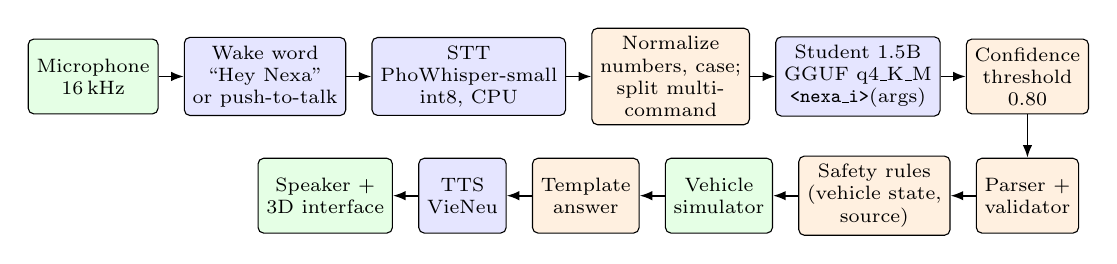
\begin{tikzpicture}[
  box/.style={draw, rounded corners=2pt, align=center, font=\scriptsize, minimum height=0.95cm, inner sep=3pt},
  model/.style={box, fill=blue!10},
  code/.style={box, fill=orange!12},
  io/.style={box, fill=green!10},
  arr/.style={-{Latex[length=1.6mm]}, semithick},
  node distance=0.32cm]
\node[io] (mic) {Microphone\\16\,kHz};
\node[model, right=of mic] (wake) {Wake word\\``Hey Nexa''\\or push-to-talk};
\node[model, right=of wake] (stt) {STT\\PhoWhisper-small\\int8, CPU};
\node[code, right=of stt] (norm) {Normalize\\numbers, case;\\split multi-\\command};
\node[model, right=of norm] (llm) {Student 1.5B\\GGUF q4\_K\_M\\\tok{nexa\_i}(args)};
\node[code, right=of llm] (thr) {Confidence\\threshold\\0.80};
\node[code, below=0.55cm of thr] (val) {Parser +\\validator};
\node[code, left=of val] (safe) {Safety rules\\(vehicle state,\\source)};
\node[io, left=of safe] (car) {Vehicle\\simulator};
\node[code, left=of car] (resp) {Template\\answer};
\node[model, left=of resp] (tts) {TTS\\VieNeu};
\node[io, left=of tts] (ui) {Speaker +\\3D interface};
\draw[arr] (mic) -- (wake); \draw[arr] (wake) -- (stt); \draw[arr] (stt) -- (norm);
\draw[arr] (norm) -- (llm); \draw[arr] (llm) -- (thr); \draw[arr] (thr) -- (val);
\draw[arr] (val) -- (safe); \draw[arr] (safe) -- (car); \draw[arr] (car) -- (resp);
\draw[arr] (resp) -- (tts); \draw[arr] (tts) -- (ui);
\end{tikzpicture}
\caption{Runtime pipeline. Blue: learned models; orange: code; green: input/output. Clarifications and refusals leave the
pipeline after the validator or safety step with a question or an apology; a pending call is executed when the driver
confirms. Everything runs on the laptop CPU; the GPU is not used.}
\label{fig:pipeline}
\end{figure*}

Figure~\ref{fig:pipeline} shows the deployed pipeline. The backend (FastAPI + WebSocket) keeps one simulated vehicle and one
pending call per session. The student runs in \code{llama-server} from llama.cpp \citep{gerganov2023llamacpp}; prompts are
sent as token ids produced by the Hugging Face tokenizer and outputs are decoded from token ids, because the text field of
the server hides control tokens such as \tok{nexa\_i}. The end-of-sequence token is overridden to \tok{nexa\_end}: without it,
uncertain refusals continued into the description seen in those 7.1\% of examples until the generation limit, which made them five to eight times
slower (identical outputs on 400 validation prompts, total time 540\,s $\rightarrow$ 249\,s).

Several small layers sit around the model; each was added after a measured failure (details in Appendix~\ref{app:runtime}):
\begin{itemize}
  \item \textbf{Text normalization.} The training data, written by the teacher, always starts with a capital letter. For
  \vi{hỏng xe giữa đường rồi}{my car broke down in the middle of the road}, the lower-case version is refused (refusal
  probability 0.68) while the capitalized one triggers a hazard-light proposal (0.99). We therefore capitalize the first
  letter, collapse repeated letters and lower-case all-caps input before the model sees it.
  \item \textbf{Retry without context.} If the model refuses while a previous turn is in the prompt, it is called once more
  without the context, so that context can help a follow-up but never turns an understood request into a refusal.
  \item \textbf{Relative-command conventions.} ``Colder'' without a number means $-2$\,°C, fan $\pm1$ level, volume $\pm3$---the
  same rules used to label the training data.
  \item \textbf{Multi-command splitting.} The training data contain no example that executes several independent actions, so
  the model picks one action from \vi{bật đèn pha lên xong kiểm tra xăng xong đó mở cốp}{turn on the headlights, then check
  the fuel, then open the trunk}. We split such utterances on explicit sequential connectors (\textit{xong}, \textit{sau
  đó}, \textit{rồi thì}, \ldots; not on \textit{và} ``and''), run the model per segment and stop at the first segment that
  needs clarification.
  \item \textbf{Answer templates.} The model was trained to phrase answers from function results, but this second pass adds
  about 1.6\,s and produced semantic errors no automatic check caught (\S\ref{sec:turn2}); the deployed system answers with
  templates filled from the result.
\end{itemize}

\subsection{Guardrails}
\label{sec:guardrails}

Following the principle ``the model understands, code keeps the car safe'', every call passes a validator and a set of
state-dependent rules declared in the function schema (Table~\ref{tab:safety}). The validator rejects values outside
enumerations or ranges, asks for missing required arguments and drops unknown arguments. Each command carries its source:
push-to-talk is treated as the driver, while the wake word can be spoken by any passenger. Mirroring a real window-lock
button, the child lock lets the driver lower rear windows directly but asks for confirmation when the request comes through
the wake word. The rules are covered by 917 automated tests, including scenario tests that, as in $\tau$-bench, check the
final vehicle state rather than the wording of the answer. We did not measure guardrails with a quantitative benchmark.

\begin{table}[t]
\centering\small
\begin{tabular}{@{}p{3.6cm}p{3.1cm}@{}}
\toprule
Condition & Action \\
\midrule
open trunk / charge port / fuel flap while driving & refuse \\
unlock doors while driving & ask to confirm \\
any sensitive function via wake word & ask to confirm \\
child lock on + wake word + rear window down or sunroof open/tilt & ask to confirm \\
driving starts with trunk, door or flap open & warn \\
model proposes a sensitive function & drop the proposal \\
\bottomrule
\end{tabular}
\caption{Runtime safety rules (code, independent of the model).}
\label{tab:safety}
\end{table}

\section{Data}
\label{sec:data}

\subsection{Distillation from a local teacher}
\label{sec:generation}

The teacher is Qwen2.5-72B-Instruct (AWQ 4-bit, \citealp{lin2024awq}) served with vLLM \citep{kwon2023vllm} on a rented A100
80\,GB; no paid API is used. For each function the teacher writes Vietnamese requests in batches of 50, extracts the call
arguments in a second pass, writes natural answers for a sample of calls given a simulated function result, and writes
out-of-scope requests that should be refused, keeping positives and refusals at about 1:1. The first pool held 27,327 samples
(about 1,000 per function) and cost about US\$13--15 of GPU time. Data is split into train and validation by groups of
near-duplicates (MinHash with a fixed hash, so the split is reproducible), so that paraphrases of the same sentence never
cross the split.

\subsection{Quality control}
\label{sec:quality}

We follow the rule ``whatever code can check, code checks'' \citep{liu2024apigen,liu2024toolace}. Code removes arguments
outside enumerations or ranges, Chinese/Japanese/Korean characters (119 samples in the first pool), leaked function names,
invented numbers in answers, mixed-English sentences and commands hidden in clarification samples. Failing samples are
discarded, not regenerated: regenerating until a judge agrees moves the judge's bias into the data.

\paragraph{Judges.}
The teacher also judges its own data, which checks consistency rather than correctness. For clarification samples we
therefore use a jury \citep{verga2024juries}: Qwen2.5-72B and Llama-3.3-70B \citep{grattafiori2024llama3} each pick up to two
functions for the sentence \emph{without seeing the label} \citep{zheng2023judging}, and a sample is kept only if both picks
contain the label. Every judging job starts with a labeled calibration set and stops if agreement in either direction is
below 80\% or Cohen's $\kappa$ below 0.6 \citep{thakur2025judging}; the jury reached $\kappa=0.875$. The previous single-judge
prompt had kept 517 of 518 clarification samples, including clearly wrong ones such as ``this parking spot looks unsafe''
$\rightarrow$ hazard lights.

\paragraph{Human audits.}
Against 400 reference labels (drafted by an LLM and corrected by the first author), the two judges agree with the reference on
the first function only 64--70\% of the time. The jury filter raises label precision from 75\% to 88\% while wrongly
discarding 16\% of correct samples. Two additional code rules (imperative particles at the end of a clause; hazard lights of
\emph{another} car), designed on one half of the 400 labels, raise precision on the other half from 86.2\% to 90.8\%. A stratified audit of 195 call/answer/refusal samples by the first author found 90.3\% correct (95\% Wilson CI 85--94),
below APIGen's 95.3\%, and exposed three systematic errors that machine judges had accepted: ``is the fuel enough for
$N$\,km'' labeled as a fuel-level query (21\% of that function), ``volume up to $N$'' labeled as a relative change (26\%), and
window direction inverted for ``close''. They were fixed by code rules in round R3. A second audit of 52 samples from round
v5 found 90.4\% correct. The lesson we drew: two machines agreeing is not evidence of correctness---Llama-3.3-70B accepted
95.2\% of the samples Qwen had approved, while a person found systematic errors in under an hour.

\subsection{Evaluation sets}
\label{sec:evalsets}

No benchmark covers Vietnamese in-car function calling with functional tokens, so we built evaluation sets that are separate
from the training pipeline in source (Table~\ref{tab:evalsets}). Sentences were generated by ChatGPT from a written description
of what the assistant can and cannot do---no example sentences and no training data were shown---and labeled by ChatGPT in a
separate conversation from a lookup table; the first author then reviewed and corrected every label. Using a different
generator from the teacher avoids the setting of Octopus~v2, where training and test queries come from the same model. We
call these sets \emph{synthetic, human-reviewed}; they are not human-written. Every set is checked against all training and
validation data and every few-shot example in the schema (MinHash near-duplicates), and frozen with a SHA-256 hash in the test
suite before any model is scored on it. The original 296-sentence test set lost 66 sentences to contamination (short car
commands are often identical), leaving the 230-sentence \emph{clean test} used throughout.

\begin{table}[t]
\centering\small
\begin{tabular}{@{}lrp{3.7cm}@{}}
\toprule
Set & $n$ & Purpose \\
\midrule
Clean test & 230 & 74 clear, 39 ambiguous, 117 out-of-scope \\
Supplement & 28 & complaints for 7 functions \\
Ambig-3 & 130 & implicit requests, 13 functions; used once \\
Ambig-4 & 129 & implicit, mostly long requests \\
v6-A / B / C & 150 & short (72), paraphrase/dialect (48), new arguments (30) \\
v6-D & 60 & two-turn follow-ups \\
v6-E & 104 & no diacritics or typos (code) \\
GRPO test & 197 & 4 parts, plus a lower-case copy \\
Calibration & 194 & hard out-of-scope, for thresholds \\
Dev & 30 & story-like requests, 20 refuse \\
\midrule
Validation & 3,416 & teacher-generated; 600 for checkpoints \\
\bottomrule
\end{tabular}
\caption{Evaluation sets. All except validation and v6-E are generated by ChatGPT from a written specification and reviewed
label by label by the first author.}
\label{tab:evalsets}
\end{table}

\subsection{Data rounds}
\label{sec:datarounds}

The training data went through six rounds; each round changed one group of factors, was diagnosed only on training statistics
and validation errors (never by reading failed test items), and was accepted or rejected by criteria written before training.
Table~\ref{tab:rounds} summarizes the rounds; \S\ref{sec:rounds} reports what they taught and Appendix~\ref{app:rounds} gives
sizes, costs and details.

\begin{table}[t]
\centering\small
\begin{tabular}{@{}lp{4.9cm}r@{}}
\toprule
Round & Main change & Train \\
\midrule
R1 & teacher pool, 1:1 refusals, balanced 300/function & 15.9k \\
R2 & synonyms per function, imperative refusals, jury for clarifications & 16.1k \\
R3 & code fixes for 3 systematic label errors & 16.0k \\
R4 & story-like refusals (rejected) + contrastive story-like calls & 17.6k \\
v5 & story-like clarifications (third contrastive pair) & 19.3k \\
v6 & short/dialect phrasing, AC delta \& mode, both rear windows, previous-turn context, typos & 28.8k \\
v6.1 & v6 + 3.3k existing refusals to restore the refusal ratio & 33.5k \\
\bottomrule
\end{tabular}
\caption{Data rounds. Side experiments (function descriptions in targets, 1,000 samples per function, a combined
configuration) are in \S\ref{sec:rounds}.}
\label{tab:rounds}
\end{table}

The final training set (v6.1) has 33,523 examples: 28,635 call targets (of which 13,778 are refusals), 3,158 clarifications and
1,730 answer-phrasing examples; 4,686 carry a previous-turn context and about 11\% (3.6k) contain removed diacritics or typos.
Refusals make up 43.3\% of call and clarification targets. Examples average 54 tokens and none exceed the 256-token limit.

\section{Training and Evaluation Protocol}
\label{sec:protocol}

\subsection{Training}
\label{sec:training}

The student is Qwen2.5-1.5B-Instruct. We use the plain Hugging Face \code{Trainer} with the loss masked by the token length of
the prompt, rather than TRL's \code{SFTTrainer}, whose completion-only collator searches for the assistant marker (which
appears twice in answer-phrasing samples) and silently masks a whole sample when it does not match. Hyperparameters follow
Octopus~v2: AdamW, learning rate $5\times10^{-5}$, 10 warm-up steps, linear decay, 3 epochs, equal loss weights for the new
tokens (Octopus~v2 found weighting unnecessary for few tokens), effective batch 16, maximum length 256, bf16. LoRA uses rank 16,
$\alpha=32$ on \code{q,k,v,o,up,down} projections; because the new tokens must be learned, \code{embed\_tokens} and
\code{lm\_head} are trained in full. Qwen2.5-1.5B ties these two matrices; saving a merged PEFT model with tied weights
silently discards the trained output layer, so we untie them before training. With the two full matrices, 480M of 2.26B
parameters are trainable (21\%). Each configuration is trained with seeds 42 and 7 on a rented A100 40\,GB, L40S or L4
(v6.1: about 57 minutes and 6,288 steps per seed). A checkpoint is saved per epoch and chosen on 600 stratified validation
samples: the highest accuracy on clear commands among checkpoints with false refusals $\le5\%$, earlier epoch on ties.

\subsection{Scoring}
\label{sec:scoring}

All models, including prompted baselines whose JSON output is converted to the functional format, are scored by the same
code. An output is \emph{correct} if it matches the reference after normalization (``rule C''): arguments equal to their
schema default are dropped on both sides (\code{get\_odometer()} = \code{get\_odometer(unit="km")}); for ambiguous items only
the function and the direction are checked (on/off, open/close, up/down, sign of a delta), and a proposal may pick any one of
several acceptable functions; suggesting the high beam is always wrong. Real behavioral differences (delta 1 vs.\ 2, miles vs.\
kilometres) are never forgiven. Rule C was fixed before round R2 and old results were re-scored with it; under the earlier
exact-match rule the same R1 outputs score 4.1 points lower on clear commands.

Errors are classified into seven types: wrong function, wrong argument, false refusal, over-triggering (calling a real
function on an out-of-scope request), unnecessary clarification, missing clarification, and unparseable output. We call
over-triggering, wrong function, wrong argument and missing clarification \emph{wrong actions}: the car would do something the
user did not ask for. We report per-group accuracy and never a single pooled number: a model that refuses everything already
scores 51\% on the clean test.

\subsection{Statistical protocol}
\label{sec:stats}

The test sets are small (74 clear commands; one item is 1.35 points), so we use Wilson intervals \citep{wilson1927} and the
exact two-sided McNemar test \citep{mcnemar1947} on paired outputs. McNemar accounts for the choice of test items but not for
training randomness: when we retrained round R2 with a second seed on identical data, 33 of 230 items changed outcome and
McNemar between the two seeds gave $p=0.005$. From then on every configuration was trained with two seeds (three for the final one, Appendix~\ref{app:seeds}), results are the
mean of the two, and a difference is claimed only if the mean difference exceeds the spread between seeds and, for paired
tests, if it is significant for both seeds in the same direction (one seed: ``tie or slightly better''). The criteria for
accepting each round, choosing thresholds and compression levels were recorded before the corresponding test run, and we
did not change them after seeing scores. Two seeds remain few; our conclusions are correspondingly modest.

\section{Results}
\label{sec:results}

\subsection{Student versus prompted baselines}
\label{sec:main}

Table~\ref{tab:main} compares the student with schema-in-prompt (SIP) baselines: the same prompt---descriptions of the
functions, the three actions, the same data policy and three examples, about 2,150 tokens---given to the untrained
Qwen2.5-1.5B-Instruct and to the 72B teacher, each run once with greedy decoding.

\begin{table*}[t]
\centering\small
\setlength{\tabcolsep}{5pt}
\begin{tabular}{@{}lccccccc@{}}
\toprule
& \multicolumn{3}{c}{Clean test (230)} & Suppl. & Ambig-4 & Prompt & p50 \\
\cmidrule(lr){2-4}
System & Clear (74) & Amb. (39) & OOS (117) & (28) & (129) & tokens & latency \\
\midrule
Qwen2.5-1.5B, prompted (SIP) & 37.8 & 35.9 & 31.6 & 14.3 & 20.9 & 2,156 & 779\,ms \\
Qwen2.5-72B teacher, prompted (SIP) & \textbf{83.8} & 56.4 & \textbf{94.9} & 39.3 & 70.5 & 2,156 & 1,842\,ms \\
\midrule
Student v5, LoRA & 78.4 & 75.6 & 83.8 & 58.9 & 78.3 & 33 & \multirow{3}{*}{224\,ms$^{\dagger}$} \\
Student v6.1, LoRA & 78.4 & 75.6 & 77.4 & 58.9 & \textbf{79.1} & 33 & \\
Student v6.1 + threshold 0.85 & 75.0 & 74.4 & 82.1 & 58.9 & \textbf{79.1} & 33 & \\
\midrule
Deployed: v6.1 s42, 4-bit, $\tau$ 0.80 & 77.0 & 64.1 & 88.0 & 50.0 & 74.4 & 33 & 520\,ms$^{\ddagger}$ \\
\bottomrule
\end{tabular}
\caption{Accuracy (\%) on the frozen evaluation sets. Student rows are means of two seeds, unquantized; baselines are single
greedy runs; OOS = out-of-scope. Latency: A100 with vLLM, one query at a time ($^{\dagger}$measured for an earlier student
with the same prompt length); $^{\ddagger}$laptop CPU, llama.cpp. The v5 row comes from the same re-generation as v6.1 and differs by at most two items per group from the original v5
run in Table~\ref{tab:lora}. The deployed row is one seed after 4-bit quantization with the threshold
(\S\ref{sec:quant}).}
\label{tab:main}
\end{table*}

\paragraph{Training is necessary.} With the same 1.5B model, prompting reaches only 14--38\% on every group (21--28\% on the
newer short, two-turn, typo and Ambig-4 sets, Table~\ref{tab:v6}); the 1.5B prompted model over-triggers on 63\% of
out-of-scope requests and returns invalid JSON for 10 clean-test items. Fine-tuning with functional tokens roughly doubles to
quadruples every group while the prompt is 65 times shorter.

\paragraph{Against the 72B teacher.} Exact McNemar tests per seed (v6.1, unquantized, Appendix~\ref{app:seeds}) give:
\emph{clear commands} 81.1 and 75.7 vs.\ 83.8 ($p=0.77$, $0.15$): no detectable difference; \emph{long implicit requests}
(Ambig-4) 79.8 and 78.3 vs.\ 70.5 ($p=0.065$, $0.14$): higher but not significant; the small ambiguous group: significant for
one seed only (tie or slightly better); \emph{out-of-scope} 82.9 and 71.8 vs.\ 94.9 ($p\le0.001$ for both): the teacher is
clearly better. On the v6 sets (Table~\ref{tab:v6}; the prompted baselines were run on them later with the same prompt and
decoding) the picture is similar: \emph{short commands and paraphrases} 88.3 and 87.5 vs.\ 91.7 ($p=0.39$, $0.27$) and
\emph{typos} 60.6 and 66.3 vs.\ 69.2 ($p=0.093$, $0.66$) are ties, \emph{new arguments} favor the student (83.3 vs.\ 70.0,
$p=0.34$), but on \emph{two-turn follow-ups} the teacher is clearly better (81.7 vs.\ 66.7 and 58.3; $p=0.049$, $0.001$),
although it never saw a two-turn example and receives exactly the previous call that the student receives. Part of the 72B's errors on clear commands are label conventions it cannot know from descriptions (an AC
temperature without \code{state="on"}, ``weak lights'' $\rightarrow$ high beam). A 1.5B model can tie a 72B one on clear and
implicit requests here because the comparison is not symmetric: the student learned this task's conventions from 33k
examples of the teacher's \emph{filtered} outputs, whereas the teacher works zero-shot from a prompt; where general knowledge
or reasoning over context is needed---recognizing what the car cannot do, or how a follow-up modifies the previous
action---the larger model remains ahead.

\subsection{What the data rounds taught}
\label{sec:rounds}

\begin{figure*}[t]
\centering
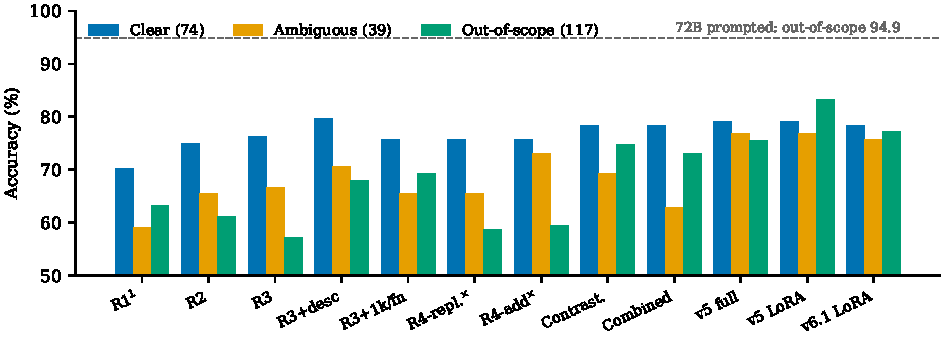
\includegraphics[width=\textwidth]{figures/rounds.pdf}
\caption{Clean-test accuracy across data configurations (means of two seeds; $^{1}$single seed; $^{\times}$rejected by
pre-registered criteria because they refused doable requests). The v6.1 row is from a later re-run of the same scorer.}
\label{fig:rounds}
\end{figure*}

Figure~\ref{fig:rounds} traces clean-test accuracy over the configurations we trained and Table~\ref{tab:ablation} gives the
side experiments on top of R3. Five findings shaped the final data.

\paragraph{Validation is not a test.} From R1 on, validation accuracy on clear commands was 97--99\%, while the clean test gave
65--80\%. Validation data come from the same teacher and prompts as training data, so they share its blind spots; only the
separately generated test sets revealed them.

\paragraph{Lexical lock-in.} In R1, 15 of 24 functions had one word covering $\ge95\%$ of their training sentences. All 267
window sentences said \textit{cửa sổ} (window) and none said \textit{kính} (glass), while every defrost sentence said
\textit{kính}; the model learned ``\textit{kính} $\Rightarrow$ defrost'' and turned \vi{Hạ kính ghế phụ}{lower the passenger
glass} into \code{set\_defrost(state="down")}. Asking the teacher to spread synonyms evenly (R2) fixed this: all nine
\textit{kính} window commands in the clean test now chose the window function, and window accuracy rose from 30\% to 80\%.

\paragraph{Shortcuts from sentence form.} R1 refusals were almost never imperative (2.1\%), so ``imperative $\Rightarrow$ call''
was 94.7\% accurate on the training data. Adding 1,667 imperative refusals in R2 broke this rule (60.4\%) but did not reduce
over-triggering (18.7\% $\rightarrow$ 17.8\%). In R4 we generated 1,651 refusals that first describe a situation and then ask
for something the car cannot do. Development-set refusals jumped from 8.5/20 to 20/20, but story-like \emph{doable} requests
were now refused (2--6 of 10, vs.\ 10/10 before): the model had learned ``story $\Rightarrow$ refuse''. Both R4 variants were
rejected by their pre-registered false-refusal criterion. Adding the same story frame on the call side (1,641 story-like calls,
the \emph{contrastive} configuration) removed the shortcut and gave the largest out-of-scope gain of the project
(57.2 $\rightarrow$ 74.8, with 10/10 doable requests kept). We now generate hard examples only in pairs across labels.

\paragraph{The same lesson for clarifications.} On a new 130-item ambiguous set (Ambig-3) with a pre-registered test, the
prompted 72B beat the contrastive student clearly (71.5 vs.\ 51.5 and 38.5; $p<0.001$ for both seeds). The student collapsed
on long, story-like complaints, mostly by refusing them. Training data explained why: among sentences longer than ten words
there were 3,254 refusals but only 102 clarifications. Round v5 added 1,696 story-like clarifications (a third contrastive
pair), judged by the jury and audited (90.4\%). On a fresh set, Ambig-4, v5 reached 74.4 and 72.1 vs.\ 51.2 and 45.0 for the
contrastive model ($p<10^{-4}$, both seeds) and became indistinguishable from the 72B (70.5; $p=0.51$, $0.87$); false
refusals on long complaints fell from 18 and 32 to 6 and 6, the 72B's level.

\paragraph{Octopus-style descriptions and data scale.} Appending function descriptions to targets raised clear commands by
3.4 points with almost no seed spread; using up to 1,000 samples per function (all of the pool) raised out-of-scope accuracy by
12 points. Combining both with the contrastive data brought no further gain: data scale and contrastive refusals fix the
same weakness, and the description effect was diluted (Table~\ref{tab:ablation}). We kept the smaller contrastive set
(17.6k vs.\ 30.0k examples) as the base for v5.

\begin{table}[t]
\centering\small
\setlength{\tabcolsep}{3pt}
\begin{tabular}{@{}lccccc@{}}
\toprule
Config. (vs.\ R3) & Clear & Amb. & OOS & Dev ref. & Dev do \\
\midrule
R3 & 76.3 & 66.7 & 57.2 & 8.5 & 10 \\
+ descriptions & \textbf{79.7} & 70.5 & 68.0 & 7.0 & 10 \\
+ 1,000 / function & 75.7 & 65.4 & 69.2 & 10.0 & 10 \\
R4 replace$^{\times}$ & 75.7 & 65.4 & 58.6 & 20.0 & 6 \\
R4 add$^{\times}$ & 75.7 & 73.1 & 59.4 & 20.0 & 2 \\
Contrastive & 78.4 & 69.2 & \textbf{74.8} & 17.5 & 10 \\
Combined & 78.3 & 62.8 & 73.0 & 16.5 & 10 \\
\bottomrule
\end{tabular}
\caption{Data experiments on top of R3 (full fine-tuning, means of two seeds). Dev ref.: refusals correct out of 20; Dev do:
doable story-like requests executed out of 10. Seed spreads are in Appendix~\ref{app:rounds}.}
\label{tab:ablation}
\end{table}

\subsection{LoRA versus full fine-tuning}
\label{sec:lora}

Octopus~v2 reports full fine-tuning slightly above LoRA (99.524\% vs.\ 99.048\%, which corresponds to one item if their test
has 210 queries). On the v5 data, with the same learning rate, seeds and selection rule, LoRA matches full fine-tuning on
clear commands and is better on out-of-scope requests (Table~\ref{tab:lora}). The out-of-scope advantage holds in all four
comparisons at equal epochs (two epochs $\times$ two seeds, +5 to +13 points); the advantage on Ambig-4 disappears at equal
epochs, so we attribute it to checkpoint choice. Full fine-tuning showed signs of overfitting (validation loss rising at
epoch 3, over-triggering growing with epochs). Lowering its learning rate to $2\times10^{-5}$ did not close the gap (76.1 on
out-of-scope; pre-registered verdict ``still behind'') and left the model under-trained on everything else. We therefore
deploy LoRA, but do not claim LoRA is better in general.

\begin{table}[t]
\centering\small
\setlength{\tabcolsep}{4pt}
\begin{tabular}{@{}lccc@{}}
\toprule
v5 data, mean of 2 seeds & Full $5\mathrm{e}{-5}$ & Full $2\mathrm{e}{-5}$ & LoRA \\
\midrule
Clear (74) & 79.1 & 71.6 & 79.1 \\
Ambiguous (39) & 76.9 & 48.7 & 76.9 \\
Out-of-scope (117) & 75.6 & 76.1 & \textbf{83.3} \\
Ambig-4 (129) & 73.3 & 46.5 & 78.3 \\
False refusal & 0.7 & 0.4 & 0.2 \\
\bottomrule
\end{tabular}
\caption{Full fine-tuning vs.\ LoRA (r\,16, $\alpha$\,32) on identical data. McNemar on the clean test: $p=0.019$ (seed 42),
$0.25$ (seed 7).}
\label{tab:lora}
\end{table}

\subsection{Short commands, context and typos (v6, v6.1)}
\label{sec:v6}

Testing the v5 demo revealed failures that the earlier test sets did not contain: terse commands (\vi{bật pha}{high beam on}
was refused), dialect words (\textit{kiếng} for \textit{kính}), missing diacritics (\vi{mo cop}{open trunk}), follow-ups
(\vi{đóng đi}{close it} after opening the trunk), relative temperature (\vi{giảm nhiệt độ điều hòa}{lower the AC temperature}
turned the AC \emph{off}, because the schema had no relative argument), and both rear windows at once. Measuring the v5
training data confirmed that teacher sentences are long and formal: only 0.7\% of call sentences have three words or fewer,
and 14 functions have none. Round v6 extended the schema (AC \code{delta} and \code{mode}, fan \code{delta}, windows
\code{front}/\code{rear}) and generated data from assigned combinations of verb, part name, abbreviation, dialect, length tier and
register, plus two-turn data with the previous call in the prompt and typos introduced by code. A new 210-item test was
written and frozen before any v6 model existed.

\begin{table}[t]
\centering\footnotesize
\setlength{\tabcolsep}{2.6pt}
\resizebox{\columnwidth}{!}{%
\begin{tabular}{@{}lccccccc@{}}
\toprule
& \multicolumn{3}{c}{Student (2 seeds)} & & \multicolumn{2}{c}{Prompted (SIP)} \\
\cmidrule(lr){2-4}\cmidrule(lr){6-7}
& v5 & v6 & v6.1 & crit. & 1.5B & 72B \\
\midrule
(1) Short + paraphrase (120) & 76.3 & 88.8 & 87.9 & pass & 27.5 & \textbf{91.7} \\
(2) Two-turn (60)$^{a}$ & 23.3 & 60.8 & 62.5 & & 28.3 & \textbf{81.7} \\
(3) New arguments (30) & 8.4 & \textbf{83.3} & \textbf{83.3} & & 16.7 & 70.0 \\
(4) Clear, old test (74) & 78.4 & 77.7 & 78.4 & pass & 37.8 & \textbf{83.8} \\
(4) Out-of-scope (117) & 83.8 & 73.1 & 77.4 & fail & 31.6 & \textbf{94.9} \\
(4) Ambig-4 (129) & 78.3 & \textbf{80.6} & 79.1 & pass & 20.9 & 70.5 \\
(5) Typos (104) & 31.7 & 64.4 & 63.5 & & 21.2 & \textbf{69.2} \\
\bottomrule
\end{tabular}}
\caption{Pre-registered comparison of the student rounds (criteria compare v6.1 with v5 only), with the prompted baselines
for reference (single greedy runs; bold = best per row). Criterion (1): better than v5 for both seeds (McNemar $p=0.0007$,
$0.007$ for v6.1); (4): no group of the old tests more than 3 points below v5. $^{a}$v5 with a rule-based memory (without
memory also 23.3); prompted baselines receive the previous call in the user message, as the student does.}
\label{tab:v6}
\end{table}

Table~\ref{tab:v6} shows a large gain on everything new and an out-of-scope regression. The training data explained it: v6
added about 9,500 mostly positive examples and the refusal share fell from 40.5\% to 33.3\%. v6.1 restored it to 43.3\% with
3,300 refusals that had already passed earlier filters (no new generation), which halved the regression ($-10.7
\rightarrow -6.4$) but still failed criterion (4), mainly because of seed 7 ($-11.1$; seed 42 $-1.7$). By our rule v6.1 does
not replace v5 as the \emph{method} result, and we report both. For the demo we nevertheless chose v6.1 seed 42, because it
handles the commands drivers actually produced in testing; seed 42 was chosen on the independent calibration set
(\S\ref{sec:threshold}), not on test scores. The rule-based memory we had written before v6 barely helped on real follow-ups
(23.3, same as no memory): human follow-ups are rarely a bare verb, whereas the model with context resolved 80--87\% of
direction changes.

\subsection{Confidence threshold}
\label{sec:threshold}

With functional tokens, the probability of the first generated token is the probability of the decision. Our rule: if the
top token is a function with $p<\tau$, refuse when the second token is the refusal token, otherwise ask the user to confirm
the full top call (so ``yes'' executes it); refusals and clarifications chosen by the model are left alone. Thresholds are
chosen on non-test data and then fixed.

\begin{figure}[t]
\centering
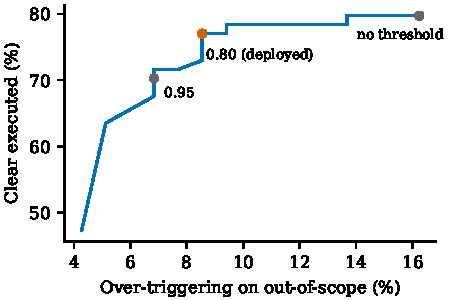
\includegraphics[width=\columnwidth]{figures/threshold.pdf}
\caption{Effect of the threshold for the deployed model on the clean test (descriptive; the threshold was chosen on the
calibration set).}
\label{fig:threshold}
\end{figure}

On the clean test the threshold consistently trades severe errors for mild ones. For the contrastive model ($\tau=0.90$,
chosen on validation) wrong actions fell from 53 to 33 and from 44 to 25 per seed (about $-40\%$); for LoRA v5 ($\tau=0.85$)
from 34/38 to 21/23; for the deployed model ($\tau=0.80$) from 41 to 29, with over-triggering on out-of-scope requests falling
from 16.2\% to 8.5\% (Figure~\ref{fig:threshold}). The price is extra confirmations: clear-command accuracy drops (e.g.\ LoRA v5
79.1 $\rightarrow$ 70.9), but every clear command lost this way was replaced by a confirmation proposing the correct call, so
the share solved after at most one ``yes'' is unchanged (59 = 52 + 7 items for seed 42). Thresholds must be re-chosen per
model: LoRA is less confident than full fine-tuning, 4-bit quantization lowers confidence further, and an under-trained model
lost every clear command at $\tau=0.90$.

Our first rule (largest $\tau$ that loses $\le1\%$ of clear commands on validation) was arbitrary, and validation contains too
few over-triggers to choose from (3--14). We therefore built a 194-sentence calibration set of hard out-of-scope requests and
asked for a guarantee: the lowest $\tau$ whose one-sided 90\% Clopper--Pearson bound \citep{clopper1934} on wrong behavior is
$\le10\%$. \emph{No model met it at any $\tau\le0.99$}: 19--28\% of these requests are handled wrongly without a threshold
and 9--16\% remain at $0.99$, because the model is confidently wrong. Separating the two kinds of error is informative:
self-executed wrong actions fall from 9--13\% to 3--5\% at $\tau=0.85$, and what the threshold cannot touch are
clarification proposals in response to chit-chat (``seeing these flame trees reminds me of school'' $\rightarrow$ ``open the
sunroof?''), a side effect of the story-like clarification data that is present in v5 and v6.1 alike. The deployed threshold
0.80 was chosen on this set (5 self-executed errors out of 194, as at 0.85, with fewer lost commands).

\subsection{Quantization and deployment}
\label{sec:quant}

The model is converted to GGUF and quantized with llama.cpp. The compression level was chosen by a rule fixed in advance on
validation and development data (3,036 items): accept the first of q4\_K\_M, q4\_K\_M+imatrix, q5\_K\_M, q8\_0 that loses at most
0.5\% of correct clear commands, adds at most two over-triggers and loses at most two ambiguous items relative to the unquantized
model. For v5, f16 conversion changed 5 of 3,036 outputs, q8\_0 5, q5\_K\_M 24 and q4\_K\_M 38; q4\_K\_M passed (q5\_K\_M failed by
one ambiguous item), so q4\_K\_M was chosen (Table~\ref{tab:quant}). llama.cpp keeps the output layer at 6 bits even in
q4\_K\_M, which protects the rows of the 27 new tokens. The f16 conversion on the same CPU reproduced the unquantized model, so
the remaining differences come from rounding, not from the hardware.

\begin{table}[t]
\centering\small
\setlength{\tabcolsep}{3pt}
\begin{tabular}{@{}lrrrrr@{}}
\toprule
v5, val+dev & Size & Clear & Over-trig. & Amb. & Same \\
\midrule
HF bf16 & 3.31\,GB & 1,506 & 14 & 127 & -- \\
f16 & 3.31\,GB & 1,508 & 14 & 126 & 3,031 \\
q8\_0 & 1.76\,GB & 1,507 & 15 & 126 & 3,031 \\
q5\_K\_M & 1.20\,GB & 1,505 & 13 & 124 & 3,012 \\
q4\_K\_M & 1.04\,GB & 1,503 & 12 & 125 & 2,998 \\
\bottomrule
\end{tabular}
\caption{Quantization of the v5 model on 3,036 validation and development items: correct clear commands, over-triggers,
correct ambiguous items and outputs identical to HF.}
\label{tab:quant}
\end{table}

\paragraph{Deployment on test.} After freezing everything, we scored the deployed v6.1 model once on all frozen sets. On
validation, q4\_K\_M had again passed the rule (+4 clear, +0 over-triggers, $-2$ ambiguous, 2,971 of 3,006 outputs identical),
yet on test it scored below the unquantized model run on GPU, most visibly on long implicit requests (Ambig-4 79.8
$\rightarrow$ 74.4) and short commands (88.3 $\rightarrow$ 82.5). To separate the effect of rounding from that of changing the
inference stack, we also converted the same model to f16 and q8\_0 GGUF and scored f16, q8\_0 and q4\_K\_M one after another on
the same CPU (Table~\ref{tab:deploy}; re-scoring q4\_K\_M reproduced all 701 earlier outputs). Two effects appear. First,
moving from batched bf16 inference on GPU to f16 on CPU already flips near-boundary items: on the small ambiguous group f16
scores 69.2 against 74.4. Second, relative to f16 on the same CPU, q4\_K\_M is significantly worse on short commands (0 vs.\ 7
flipped items, $p=0.016$) and close to significant on Ambig-4 (1 vs.\ 7, $p=0.070$), whereas q8\_0 gives the same output as
f16 for 680 of 701 prompts and differs significantly on no group. Validation items are confident (top-token probability near
0.99), so small numeric shifts rarely flip them; the human-reviewed sets contain many near-boundary decisions that do. We keep
q4\_K\_M because the choice was made by a fixed rule on non-test data, and note that this rule is not sensitive enough to
distribution shift. q8\_0 is the safer choice on stronger hardware: it is 1.7$\times$ larger and, in the same session, 1.8$\times$
slower than q4\_K\_M (median 856 vs.\ 463\,ms). With the threshold, all three levels make the same number of wrong actions on
the clean test (29). On the laptop CPU (i5-12500H, 8 threads) the deployed model needed 520\,ms at the median and 961\,ms at
the 95th percentile per decision in the first scoring session (463 and 832\,ms in the second).

\begin{table}[t]
\centering\small
\setlength{\tabcolsep}{2.5pt}
\resizebox{\columnwidth}{!}{%
\begin{tabular}{@{}lccccc@{}}
\toprule
v6.1 seed 42 & HF (GPU) & f16 & q8\_0 & q4 & q4 + 0.80 \\
\midrule
Clear (74) & 81.1 & 81.1 & 81.1 & 79.7 & 77.0 \\
Ambiguous (39) & 74.4 & 69.2 & 69.2 & 64.1 & 64.1 \\
Out-of-scope (117) & 82.9 & 82.1 & 82.1 & 82.9 & 88.0 \\
Ambig-4 (129) & 79.8 & 79.1 & 78.3 & 74.4 & 74.4 \\
Short + paraphr.\ (120) & 88.3 & 88.3 & 85.0 & 82.5 & 79.2 \\
Two-turn (60) & 66.7 & 66.7 & 65.0 & 61.7 & 56.7 \\
Typos (104) & 60.6 & 58.7 & 60.6 & 55.8 & 47.1 \\
Wrong actions, clean & 37 & 40 & 40 & 41 & 29 \\
Median latency (CPU) & -- & 1,062 & 856 & 463 & 463 \\
\bottomrule
\end{tabular}}
\caption{The deployed model (v6.1 seed 42) on the frozen test sets. HF: unquantized, batched bf16 on GPU. The other columns
are GGUF on the same laptop CPU in one session; latency in ms per decision (p95: 2,075 / 1,480 / 832). The threshold does not
change the model's own clarifications, so the ambiguous rows of the last two columns are identical.}
\label{tab:deploy}
\end{table}

\paragraph{Answer phrasing.}
\label{sec:turn2}
The model can also phrase the answer from the function result (second prompt). Measured with the v5 model on 200 validation
samples, it refused
correctly in 99 of 99 out-of-scope samples, and 87.1\% of informative answers passed the code checks (no invented number, no
English words), but it also produced semantic errors that no check caught (``today'' for a two-day forecast, a wrong pressure
comparison) and added a median 1.6\,s. The deployed system therefore answers with templates; model answers remain available
as an option.

\subsection{GRPO after distillation}
\label{sec:grpo}

Since the remaining errors are decisions (call, clarify or refuse), we tried GRPO \citep{shao2024deepseekmath} with a
code-computed reward that weights errors by their consequence: correct $+1$, unnecessary clarification $-0.2$, false refusal or
wrong proposal $-0.5$, unparseable $-1$, wrong action on the car $-5$. The magnitude $-5$ is tied to the runtime threshold:
acting at $p=0.8$ has the same expected reward as asking ($0.8\cdot1-0.2\cdot5=-0.2$). A fresh LoRA (r\,16) on the merged
v6.1 model was trained with TRL, $G=8$, learning rate $10^{-5}$, KL coefficient 0.04 and temperature 1.0 for two epochs on
about 4,000 training prompts on which v6.1 was uncertain ($p_{\text{top}}<0.95$, including lower-cased copies) plus 400
confident ones. A new 200-item test set (197 after removing 3 contaminated items, plus a lower-cased copy) was frozen before
training, together with five acceptance criteria.

\begin{table}[t]
\centering\small
\begin{tabular}{@{}lccc@{}}
\toprule
Criterion (mean of 2 seeds) & v6.1 & GRPO & \\
\midrule
(1) Wrong actions $\downarrow$ & \textbf{6.3\%} & 6.9\% & fail \\
(2) Implicit (M) & 80.1 & 81.2 & pass \\
(3) Clear (R) & 85.0 & 85.0 & pass \\
(4) False refusals $\downarrow$ & 1.3\% & \textbf{0.6\%} & pass \\
(5) Unneeded clarif.\ in R & 0.0 & 0.0 & pass \\
\bottomrule
\end{tabular}
\caption{GRPO vs.\ its starting point on the GRPO test set (original and lower-cased copies). GRPO had to reduce wrong actions
without hurting the other criteria.}
\label{tab:grpo}
\end{table}

GRPO failed the main criterion (Table~\ref{tab:grpo}). It barely changed the model: at the end of training 81--87\% of the
8-sample groups had identical rewards (no learning signal), the largest weight change in a query projection was
$2.4\times10^{-4}$, and only 1--16 of 197 items changed outcome per evaluation. Seven items flipped from correct to a wrong
action (unsupported features close to real ones, such as ``honk the horn'' or ``lane-departure warning'') and three in the
other direction, a difference within noise. GRPO did improve what it practiced: 60\% of the uncertain prompts were lower-cased
copies, and false refusals on lower-cased input fell from 8 to 3 for one seed---a problem the runtime already solves by
capitalization. Compared with tool-use RL that succeeds \citep{qian2025toolrl,zhang2025tooln1}, our setting lacks a reasoning
step (the decision is one token, so sampling explores little), and our prompts were already solved by the model, whereas DAPO
\citep{yu2025dapo} continuously filters such groups. We keep v6.1 and report GRPO as a negative result (cost about US\$2.2).

\section{Speech Interface}
\label{sec:speech}

Voice is the primary interface; typing is a fallback. Speech recognition (STT) and synthesis (TTS) run in a separate local
service. TTS is used off the shelf. STT was first used off the shelf (\S\ref{sec:stt}--\ref{sec:noise}); the deployed
recognizer is a version fine-tuned on car commands (\S\ref{sec:sttft}).

\subsection{Recognition, numbers and end-to-end accuracy}
\label{sec:stt}

\paragraph{Setup.} Candidates were Parakeet-CTC-0.6B-Vietnamese \citep{nvidia2026parakeetvi} (exported to ONNX, int8),
PhoWhisper-small and PhoWhisper-medium \citep{le2024phowhisper} (CTranslate2 int8 via faster-whisper), all on 8 CPU threads
with greedy decoding. TTS is VieNeu-TTS \citep{vieneu2026tts} (0.1B, 48\,kHz, ONNX on CPU, female northern voice). The
recognizers write numbers as words (\textit{hai mươi hai độ}, ``twenty-two degrees''), whereas the student was trained on
digits, so transcripts go through a normalizer that converts spoken numbers to digits, removes final punctuation and
capitalizes the first letter. The end-to-end metric is: speech $\rightarrow$ STT $\rightarrow$ normalizer $\rightarrow$
deployed model $\rightarrow$ rule-C scoring against the frozen reference, alongside the same chain fed with the original
text (``typed''). Set A (230 clean-test sentences read by 25 synthetic voices) served only for debugging; sets B, C and D
(40, 30 and 30 sentences sampled from frozen test sets, each list locked before reading) were recorded by the first author with
a laptop microphone in a quiet room.

\begin{table}[t]
\centering\small
\setlength{\tabcolsep}{3.5pt}
\begin{tabular}{@{}lcccc@{}}
\toprule
Set B (40, real voice) & Correct & WER & p50 & p95 \\
\midrule
Typed (same chain) & 30 & -- & -- & -- \\
Parakeet-CTC 0.6B & 15 & 33.3 & 388\,ms & 489\,ms \\
PhoWhisper-small & \textbf{21} & 20.2 & 1,844\,ms & 4,716\,ms \\
PhoWhisper-medium & 18 & \textbf{17.0} & 4,806\,ms & 5,136\,ms \\
\bottomrule
\end{tabular}
\caption{STT selection (pre-registered rule: most end-to-end correct; within two items, lower p95 latency). Measured before
the number-normalization fix.}
\label{tab:stt}
\end{table}

\paragraph{Choosing the recognizer.} PhoWhisper-small won the pre-registered comparison (Table~\ref{tab:stt}).
PhoWhisper-medium had the lowest word error rate but fewer correct commands: WER weighs every word equally, while one wrong
number or part name breaks a command (medium heard ``25 degrees'' as \textit{hai găm độ}). Synthetic speech overrated
Parakeet (WER 21.5\% on set A, 33.3\% on real voice): the CTC model glues or splits syllables on real speech, while the
Whisper decoder uses linguistic context.

\paragraph{A bug found by real voice.} Of the 11 commands PhoWhisper-small lost on set B, three were caused by our own
normalizer: Vietnamese speakers say \textit{hai hai độ} for 22 degrees, and the normalizer added the digits (4 degrees). After
the fix, a new set C gained four commands (17 $\rightarrow$ 21 of 30), all colloquial numbers; set A, read by TTS voices that
pronounce numbers in full, did not change at all. Re-scoring set B after the fix (22 of 40) is reported only as post-hoc.
Vocabulary hints and beam search were then compared on a new set D under a pre-registered rule: greedy without hints scored
17, hints 16, beam 5 17, both 16, so greedy was kept.

\paragraph{End-to-end.} The headline numbers for the off-the-shelf recognizer pool the 60 new sentences of sets C and D:
\textbf{42 of 60 (70.0\%) typed and 38 of 60 (63.3\%) spoken}, so speech costs 6.7 points. Per set the drop was 22.5 points on B (before the
fix), 10 on C and 3.3 on D. For context, SFC-Bench reports drops of 17--20 points for 8B--32B models at its easiest level
\citep{peng2026sfc}; the settings differ in language, functions, metric and speech (synthetic there, one real speaker here),
so we place our numbers in that range rather than compare them. The remaining speech errors are real mishearings---n/l and
tr/ch confusions (\textit{Nội Bài} $\rightarrow$ \textit{lộ tài}), \textit{độ} (degree) $\rightarrow$ \textit{đội}---which the
model mostly handles by refusing or asking rather than acting.

\subsection{Noise robustness}
\label{sec:noise}

All recordings were made in a quiet room, and the system has no denoising stage. With the off-the-shelf recognizer, we mixed the 60 C+D recordings with three
noises at 20, 10, 5 and 0\,dB SNR relative to the speech portion: real in-car noise (DEMAND \code{TCAR}, \citealp{thiemann2013demand}),
synthetic brown noise and Vietnamese background speech from FLEURS \citep{conneau2023fleurs}. The pre-registered rule was to try a
denoiser only if in-car noise at 10\,dB cost more than 6 of 60 commands.

\begin{figure}[t]
\centering
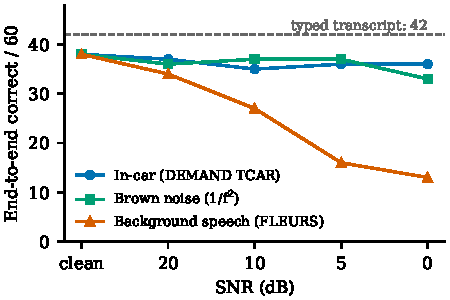
\includegraphics[width=\columnwidth]{figures/noise.pdf}
\caption{End-to-end correct commands (of 60) under additive noise.}
\label{fig:noise}
\end{figure}

In-car noise at 10\,dB cost 3 commands, so no denoiser was added (Figure~\ref{fig:noise}). PhoWhisper's WER stayed at about 22\% for
in-car noise down to 0\,dB; differences of one to three commands are within noise for 60 items. The real weakness is
\emph{another person speaking}: at 10\,dB the chain lost 11 commands, and at 5\,dB the recognizer transcribed the background
speaker as well (WER above 100\%), leaving 1 of 35 clear commands. The failure is safe: out-of-scope items stayed at 10--11 of
12, because the model refuses garbled text instead of acting on it. Single-channel denoisers target stationary noise and cannot
separate a second voice; multi-microphone hardware or source separation would be needed. Music was not tested. Separately,
browser audio processing (noise suppression and automatic gain) removed high-frequency consonants in the demo
(\vi{nóng quá}{so hot} heard as \textit{lóng quá}); requesting raw audio made the demo match the measured condition.

\subsection{Improving recognition}
\label{sec:sttft}

In live use the recognizer felt worse than the measured 63\%, so we looked for the cause and for a remedy, reusing the
recordings. Every remedy was selected on set B and checked on other data under a rule written down beforehand; sets C and D
were reused three times in this subsection and are therefore not used for the final numbers.

\paragraph{The demo's audio path is not the cause.} We replayed the 60 C+D recordings through the real interface: Chromium
used each file as a fake microphone, the page recorded it with \code{MediaRecorder} (WebM/Opus) and posted it to the same
service. The chain was correct on 36 of 60 commands, against 38 when the WAV files were sent directly (exact McNemar
$p=0.63$); half of the transcripts differed, but in both directions. The recognizer itself is the bottleneck: it misrecognizes
22\% of the words even on the original files, and tiny changes in the audio change its output.

\paragraph{Three training-free remedies did not help.} (i) A different recognizer: Zipformer-30M
\citep{yao2023zipformer,hynt2025zipformervi}, a 30M-parameter transducer run with sherpa-onnx, was ten times faster (median
0.17\,s vs.\ 1.75\,s) and had a lower WER (15.7\% vs.\ 22.0\% on C+D), yet produced \emph{fewer} correct commands (20 vs.\ 22
on B; 32 vs.\ 38 on C+D, $p=0.18$). Its errors fall on the words that select a function---\textit{nắp xăng} (fuel flap)
$\rightarrow$ \textit{lắp sang}, \textit{cốp} (trunk) $\rightarrow$ \textit{cúp}---whereas PhoWhisper's fall on sentence-final
particles and filler words that the language model ignores. It failed the pre-registered rule (three more correct commands
on B); a rule relaxed after seeing set B (lower WER, not significantly worse) would have admitted it, but with fewer correct
commands on both sets we kept PhoWhisper. As with PhoWhisper-medium above, average WER is the wrong yardstick for spoken
commands. (ii) Running both recognizers and keeping the transcript on which the language model is more
confident gave exactly PhoWhisper's score (22 of 40; 38 of 60), although an oracle choice would reach 25 and 42: the
decision-token confidence tells whether a sentence is a clear command, not whether it was heard correctly, so the model is
just as confident on \textit{lắp sang}. (iii) Repairing misheard multi-syllable part names with the initial-consonant
confusions common across Vietnamese regions (l/n, s/x, ch/tr, d/gi/r), from a vocabulary written before any recording, changed
three PhoWhisper transcripts and no outcome (on 30,060 accented training sentences it altered 0.37\%, mostly injected
typos).

\paragraph{Fine-tuning the recognizer.} We then fine-tuned PhoWhisper-small on in-domain audio: 5,000 command sentences from
the language model's \emph{training} data (contamination-checked against all test sets and recording sets), with digits
spelled out and read by 23 of the 25 VieNeu voices; 1,500 FLEURS training utterances to preserve general Vietnamese; and, for
variant B only, 150 new sentences read by the first author (12 minutes, repeated four times). Each sample is degraded at
random while training: speed 0.9--1.1, synthetic reverberation, DEMAND in-car noise at 0--20\,dB SNR, a laptop-microphone
band-pass and gain. Training takes three epochs at learning rate $10^{-5}$ (6--8 minutes on an A100); each epoch is converted
to the same CTranslate2 int8 format, so latency is unchanged. The checkpoint was chosen on set B (ties by lower WER) and
evaluated once on a new 40-sentence set E recorded for this purpose; forgetting was checked on 300 FLEURS test utterances and on
set G, 60 frozen-test commands read by the two VieNeu voices held out from training.

\begin{table}[t]
\centering\small
\setlength{\tabcolsep}{3.2pt}
\begin{tabular}{@{}lcccc@{}}
\toprule
& Set B & \multicolumn{2}{c}{Set E (final)} & FLEURS \\
\cmidrule(lr){3-4}
Recognizer & /40 & /40 & WER & WER \\
\midrule
Typed (same chain) & 30 & 32 & -- & -- \\
PhoWhisper-small & 22 & 24 & 24.8 & 11.6 \\
\quad + TTS and FLEURS (A) & 23 & 25 & 21.2 & 10.7 \\
\quad + 12 min real voice (B) & \textbf{25} & \textbf{28} & \textbf{14.5} & 10.8 \\
\bottomrule
\end{tabular}
\caption{Fine-tuning the recognizer: end-to-end correct commands with the deployed language model, and word error rate
(\%). Set B selected the checkpoint; set E was used once.}
\label{tab:sttft}
\end{table}

Table~\ref{tab:sttft} shows that synthetic speech alone barely helps on a real voice (and raised wrong actions on set E from
6 to 9), while adding 12 minutes of real recordings cuts the word errors by 40\% and recovers half of the gap to typed input
(24 $\rightarrow$ 28 of 32), with wrong actions unchanged at 6. What the off-the-shelf recognizer lacked was therefore
acoustic---this voice and this microphone---rather than vocabulary. Variant B is deployed. Three cautions apply. The gain on
set E is five commands won and one lost ($p=0.22$), not significant with 40 items, though consistent with set B. Set E shares
its speaker, microphone and recording session with the fine-tuning recordings, so it measures the benefit for \emph{this}
speaker. And for other speakers we could only show absence of harm: FLEURS WER did not rise, and on set G correct commands
went from 29 to 46 of 60 for both variants---a figure inflated by the shared TTS engine, which we read only as ``no harm''. A
check on other real speakers giving commands is missing; the noise and wake-word experiments were run with the original
recognizer.

\subsection{Wake word}
\label{sec:wake}

``Hey Nexa'' lets the driver start a command hands-free. Porcupine's free tier is no longer available and running STT
continuously costs about 1.8\,s of CPU per utterance, so we trained a detector on openWakeWord's
\citep{scripka2023openwakeword} frozen feature extractors (mel spectrogram and a speech embedding model,
\citealp{lin2020kws}): 16 frames of 96 dimensions (1.28\,s) feed a small scikit-learn MLP, updated every 80\,ms. A detection
requires $k$ consecutive frames above a threshold, followed by a 2\,s refractory period; Silero VAD \citep{silero2024vad} ends the
command after silence, and the wake phrase is stripped from the transcript. Wake-word commands carry the source
\code{wake\_word}, which activates the confirmation rules of Table~\ref{tab:safety}; the detector pauses while the assistant
speaks.

Version 1 used only synthetic positives (VieNeu reading six Vietnamese spellings of ``hey nexa'' with 20 voices, 5 held out),
synthetic negatives (near-miss phrases, car commands, the assistant's own replies), Vietnamese FLEURS training audio and 500k
precomputed ACAV100M feature windows \citep{lee2021acav100m}. It caught 98.9\% of held-out synthetic calls but only 16 of 40 of
the first author's real calls. The recordings peaked at $-23$ to $-38$\,dBFS, whereas training positives peaked at $-18$ to $-3$\,dBFS, and fast calls rarely stayed
above threshold for the required four frames. Version 2 widened the level augmentation to $-46\ldots-3$\,dB, added 46 real
training calls (14 held out for validation, none from the test recordings), and re-selected $k$ and the threshold on
validation.

\begin{table}[t]
\centering\small
\setlength{\tabcolsep}{4pt}
\begin{tabular}{@{}lccc@{}}
\toprule
& v1 & v2 & Target \\
\midrule
Real calls detected (40, new set) & 16$^{a}$ & \textbf{39} & $\ge$36 \\
False alarms / h (FLEURS test, 3.15\,h) & \textbf{1.27} & 2.86 & $\le$1 \\
Triggers on 30 spoken car commands & -- & 1 & 0 \\
Self-wake on assistant replies (38) & 0 & 0 & 0 \\
\bottomrule
\end{tabular}
\caption{Wake-word test (each measured once). $^{a}$On the first recording set. Rules: v1 four frames $\ge0.05$; v2 three
frames $\ge0.85$. CPU: about 3.5\% of one core.}
\label{tab:wake}
\end{table}

Version 2 detects almost every real call in every style (normal, fast, quiet, from 1--1.5\,m, with \textit{ơi}, followed
directly by a command), but false alarms doubled on continuous read speech, and one of the author's car commands triggered it
(Table~\ref{tab:wake}). We deploy version 2 and report that it meets the detection target but not the false-alarm target. A false
wake-up either times out after about four seconds of silence or sends the next overheard sentence to the assistant, which
usually refuses it; sensitive functions always require confirmation for wake-word commands. Because ACAV100M features are
licensed CC BY-NC-SA, the detector may only be used non-commercially.

\subsection{Latency}
\label{sec:latency}

On the laptop CPU a spoken command takes about 2.5\,s from end of speech to the start of the spoken answer: STT about 1.8\,s
for a 2--5\,s utterance, the model about 0.5\,s, and TTS about 0.25\,s until the first audio. The answer is synthesized and
streamed chunk by chunk, and the interface plays each chunk while the next one is generated. On ten answers this cut the time
to first audio from a median of 798\,ms (worst 2.8\,s for a three-part answer) when waiting for the whole sentence to 241\,ms
(worst 285\,ms). Synthesis runs faster than playback (0.85\,s for 2.7\,s of audio), so chunks play without gaps. Each extra
segment of a multi-command utterance adds about 0.5\,s. The laptop's 4\,GB GPU is not used.

\section{Discussion}
\label{sec:discussion}

\paragraph{Where the small model stands.} On the commands a car assistant mostly receives, the 1.5B student is statistically
indistinguishable from the 72B teacher while being 65 times cheaper in prompt length, about eight times faster on the same GPU
and small enough for a laptop CPU. Its consistent weakness is knowing what it \emph{cannot} do: unsupported features that
resemble supported ones (``honk'', ``lane-departure warning'', ``left turn signal'' $\rightarrow$ hazard lights at $p=0.99$)
are mapped to the nearest real function, often with high confidence. Data helps (contrastive refusals, more samples) and a threshold helps against uncertain mistakes, but
neither removes confidently wrong decisions; this matches the over-triggering reported for functional tokens by
\citet{jafarzadeh2026fixedkeys}. A hybrid design that forwards uncertain requests to a larger model when a connection is
available is the natural next step for a product.

\paragraph{Form sensitivity is a distillation artifact.} The student reacts to surface form that carries no meaning:
lower-casing only the first letter of the 230 clean-test sentences raised false refusals of the v5 model from 3 to 21, and a
lower-case
\vi{hỏng xe giữa đường rồi}{my car broke down} was refused while the capitalized version was understood. The teacher writes
clean, capitalized, formal sentences, and sequence-level distillation transfers only what appears in the data. The same cause
explains the gap between validation (97--99\%) and the independently generated tests (75--88\%), the lexical lock-in of R1, and
the need for short and noisy data in v6. Diversity has to be designed into generation (assigned personas, contexts, lengths
and vocabulary), because asking the teacher to ``write many varied sentences'' does not produce it.

\paragraph{Shortcuts appear wherever a feature is one-sided.} Three times a feature of sentence form ended up on one side of
the label distribution---imperative mood on calls (R1), stories on refusals (R4), long sentences on refusals rather than
clarifications (before v5)---and each time the model learned it as a rule. Adding hard examples in contrastive pairs across
labels was the single most effective data intervention we found. A test set of mostly short commands did not reveal the R4
shortcut; only a development set containing story-like \emph{doable} requests did.

\paragraph{Measurement discipline changed conclusions.} Several results looked like improvements and were not: R2's gain on
the ambiguous group was one lucky seed; the ``student beats 72B on ambiguity'' impression came from a 39-item group and
reversed on 130 items; the threshold's cost on clear commands was 6--10 times larger on test than on validation; 4-bit
quantization passed on validation and lost five points on implicit requests at test time. Freezing test sets before scoring,
training two seeds, testing paired outputs and writing criteria down in advance was cheap compared with the cost of drawing
these wrong conclusions.

\paragraph{When RL helps.} GRPO needs prompts on which the policy sometimes succeeds and sometimes fails, and benefits from a
reasoning step that offers several paths to sample. A functional-token model trained by distillation offers neither: its
decision is one token, and most training prompts are already solved. RL on fresh, harder prompts or a preference method on
explicitly paired outputs \citep{ross2025when2call} would be better matched to this setting; we did not run either.

\section{Conclusion}
\label{sec:conclusion}

Nexa Drive shows that a 1.5B model with functional tokens, distilled from an open 72B teacher with about US\$100 of rented GPU
time, can serve as a Vietnamese in-car assistant on a laptop CPU: it handles clear and implicit requests about as well as the
prompted teacher, asks instead of guessing when a request is only a complaint, and is wrapped in code that keeps wrong
decisions away from the car. The project's main lessons are about data and measurement rather than architecture: hard examples
must be added in contrastive pairs, synthetic validation data hides the weaknesses that matter, and small test sets need
several seeds and paired tests before a difference is believed. The remaining weaknesses---refusing unsupported features,
sensitivity to quantization on ambiguous input, background speech, and false wake-ups---are measured and documented, and
define the next steps: real-user data, a hybrid on-device/cloud design and multi-microphone input.

\section*{Limitations}

\paragraph{Synthetic evaluation.} All language test sets were generated by ChatGPT from a written specification and reviewed by
one person, the first author, who also saw the draft labels. They are separate from the training generator but are still LLM
text: real drivers speak more tersely, hesitate and make requests no specification anticipates. Absolute accuracies may
therefore be optimistic; comparisons between systems scored on the same sets are more reliable. The two reviewed label sets
used to measure the judges (ChatGPT and Claude drafts) were corrected by the same person, so we have no independent
human--human agreement baseline.

\paragraph{Small sets and repeated use.} Groups contain 28--150 items and the clean test was used across many rounds; v6 and
v6.1 were two attempts on the same test, and the Ambig-3 set was retired after one use. We trained only two seeds per
configuration. Differences below about five points should be read as unresolved.

\paragraph{One speaker, quiet room.} All real recordings (STT sets, wake-word training and test calls) come from the first
author on a laptop microphone. Noise was added digitally from recordings, not captured while driving; music was not tested. The
wake word was trained partly on the author's voice and may detect other speakers less reliably; it is not speaker
verification.

\paragraph{Scope.} The vehicle is simulated; navigation, nearby search and weather return simulated results. The system is
Vietnamese only (an English extension was planned but not done). The model cannot execute several independent actions in one
call---multi-command utterances are split by connector words at runtime, and requests joined by \textit{và} (``and'') still
lead to a single action. Answers are template-based by default.

\paragraph{Thresholds and quantization.} The threshold and the compression level were chosen on data whose distribution
differs from the tests; on test, the threshold cost more clear commands and quantization more ambiguous items than validation
predicted. No model could be certified to keep wrong behavior below 10\% on the calibration set.

\paragraph{Guardrails.} The safety rules are tested by scenario tests but not measured on a benchmark; they cover a handful of
state conditions and do not include cross-component rules (e.g.\ AC and windows), weather or emergency hand-over.

\section*{Ethics Statement}

The assistant cannot steer, brake or accelerate; actions that open the car are refused while driving and confirmed when
requested through the wake word. Voice recordings are of the first author only, who consented to their use. External data are
used under their licenses: FLEURS and DEMAND (CC BY 4.0), ACAV100M features (CC BY-NC-SA 4.0, which restricts the wake-word model
to non-commercial use), the Khronos \emph{Car Concept} 3D model (CC BY 4.0). VieNeu-TTS embeds an inaudible watermark in synthetic
speech. ChatGPT was used to generate evaluation sentences and draft labels, which were reviewed by a person. An AI assistant
(Claude) was used for code assistance and to draft this report from the project log; all reported numbers were checked against
the experiment output files.

\section*{Acknowledgments}

We thank the Faculty of Information Technology of Hung Yen University of Technology and Education. GPU time was rented from
Modal; the total cost of data generation, training and evaluation was about US\$100.


\bibliography{references}

\appendix
\section{Function Inventory}
\label{app:functions}

Table~\ref{tab:fullfunctions} lists the 24 functions with their arguments (\code{?} optional). Read-only functions (R) are
never clarified; sensitive functions (S) are never proposed from an implicit request and require confirmation from the wake
word.

\begin{table*}[t]
\centering\small
\begin{tabular}{@{}rlp{10.4cm}c@{}}
\toprule
Token & Function & Arguments & \\
\midrule
0 & \code{get\_fuel\_level} & -- & R \\
1 & \code{get\_battery\_range} & -- & R \\
2 & \code{get\_tire\_pressure} & \code{wheel?} $\in$ \{front\_left, front\_right, rear\_left, rear\_right\} & R \\
3 & \code{get\_vehicle\_status} & -- & R \\
4 & \code{get\_odometer} & \code{unit?} $\in$ \{km, mi\} & R \\
5 & \code{get\_range\_estimate} & \code{trip\_km?} $\ge 0$ & R \\
6 & \code{set\_ac} & \code{state} $\in$ \{on, off\}, \code{temperature?} 16--30, \code{zone?} $\in$ \{driver, passenger, rear, all\},
\code{delta?} $-14$..14, \code{mode?} $\in$ \{cool, heat, auto\} & \\
7 & \code{set\_fan\_speed} & \code{level?} 0--7 or \code{delta?} $-7$..7 (exactly one) & \\
8 & \code{set\_defrost} & \code{state} $\in$ \{on, off\}, \code{zone?} $\in$ \{front, rear, both\} & \\
9 & \code{lock\_doors} & -- & \\
10 & \code{unlock\_doors} & \code{door?} $\in$ \{driver, passenger, rear\_left, rear\_right, all\} & S \\
11 & \code{open\_trunk} & -- & S \\
12 & \code{close\_trunk} & -- & \\
13 & \code{open\_charge\_port} & -- & S \\
14 & \code{open\_fuel\_flap} & -- & S \\
15 & \code{control\_window} & \code{window} $\in$ \{front\_left, front\_right, rear\_left, rear\_right, front, rear, all\},
\code{position} $\in$ \{up, down\}, \code{amount?} 0--100 (default 100) & \\
16 & \code{operate\_sunroof} & \code{action} $\in$ \{open, close, tilt\}, \code{intensity?} 0--100 & \\
17 & \code{set\_headlights} & \code{mode} $\in$ \{off, auto, low\_beam, high\_beam, parking\} & \\
18 & \code{set\_hazard\_lights} & \code{state} $\in$ \{on, off\} & \\
19 & \code{set\_volume} & \code{set\_value?} 0--40 or \code{delta?} $-40$..40 (exactly one) & \\
20 & \code{play\_media} & \code{source?} $\in$ \{radio, bluetooth, usb, streaming\}, \code{query?} & \\
21 & \code{navigate\_to} & \code{destination}, \code{avoid?} $\in$ \{none, tolls, highways\} & \\
22 & \code{find\_nearby} & \code{category} $\in$ \{gas\_station, charging\_station, parking, restaurant, hospital, atm, coffee\},
\code{radius\_km?} 0.5--25 & \\
23 & \code{get\_weather} & \code{location?}, \code{day?} 0--6 & R \\
24 & \code{irrelevant\_function} & -- (refuse) & \\
\bottomrule
\end{tabular}
\caption{Function signatures of the final schema (v6). \code{delta}/\code{mode} of \code{set\_ac}, \code{delta} of
\code{set\_fan\_speed} and the \code{front}/\code{rear} windows were added in round v6, appended at the end of the argument list so
that older positional calls keep their meaning.}
\label{tab:fullfunctions}
\end{table*}

\section{Prompts and Outputs}
\label{app:prompts}

\paragraph{Call prompt (turn 1).} The system message reads \textit{Bạn là tác tử điều khiển xe ô tô.} (``You are an agent that
controls a car.'').
\begin{Verbatim}[fontsize=\small]
<|im_start|>system
Bạn là tác tử điều khiển xe ô tô.<|im_end|>
<|im_start|>user
Bật điều hòa 22 độ ghế lái<|im_end|>
<|im_start|>assistant
\end{Verbatim}
Training target (in most examples it ends here; 7.1\% additionally continue with a function description after
\tok{nexa\_end}, which is never used at inference):
\begin{Verbatim}[fontsize=\small]
<nexa_6>(state="on", temperature=22,
  zone="driver")<nexa_end>
\end{Verbatim}
Optional continuation: \code{Mô tả hàm: Bật hoặc tắt điều hoà, \ldots} (``function description: turn the AC on or off\ldots'').

\paragraph{Two-turn prompt (v6 on).} The user turn starts with the last executed call; read-only calls are not carried over.
\begin{Verbatim}[fontsize=\small]
Lượt trước: <nexa_15>(window="front_right",
  position="down", amount=100)
Bên trái phía trước cũng vậy luôn nha.
\end{Verbatim}
(``Previous turn: lower front-right window. Do the same for the front left.'') $\rightarrow$
\begin{Verbatim}[fontsize=\small]
<nexa_15>(window="front_left",
  position="down", amount=100)
\end{Verbatim}

\paragraph{Clarification and refusal.}
\vi{Trong xe bí quá}{it is stuffy in the car} $\rightarrow$ two proposals separated by a semicolon, rendered as ``Turn on the AC
or lower the windows?'':
\begin{Verbatim}[fontsize=\small]
<nexa_ask><nexa_6>(state="on");
<nexa_15>(window="all",
  position="down")<nexa_end>
\end{Verbatim}
\vi{Bạn có thể giúp tôi sửa xe được không}{can you fix my car} $\rightarrow$ \tok{nexa\_24}\code{()}\tok{nexa\_end}.

\paragraph{Answer prompt (turn 2).} The call is followed by a \code{tool} turn holding the JSON result; the target is a
Vietnamese sentence written by the teacher that may only use numbers present in the result.

\paragraph{Schema-in-prompt baseline.} The baseline prompt (2,156 tokens) contains the descriptions and arguments of the 23
functions, the three allowed JSON actions (\code{call}, \code{clarify}, \code{refuse}), the same data policy as the training data
(no clarification for read-only functions, no proposal of sensitive functions, only stated arguments) and three examples that
do not occur in any test set. Outputs are converted to the functional format; invalid JSON or unknown functions are scored as
unparseable.

\section{Data Rounds in Detail}
\label{app:rounds}

\begin{table*}[t]
\centering\small
\setlength{\tabcolsep}{4pt}
\begin{tabular}{@{}lrp{8.0cm}ccc@{}}
\toprule
Config.\ & Train & Change (diagnosis from training statistics or validation) & Clear & Amb. & OOS \\
\midrule
R1 & 15,942 & pool of 27k teacher samples, 300 per function, 1:1 refusals & 70.3$^{1}$ & 59.0$^{1}$ & 63.2$^{1}$ \\
R2 & 16,080 & synonyms (\code{tu\_dong\_nghia}) for 15 functions, 1,667 imperative refusals, jury-filtered clarifications,
situation guidance for 6 thin functions & 75.0 (4.0) & 65.4 (12.8) & 61.1 (7.7) \\
R3 & 16,010 & code fixes: fuel range, volume target, window direction, duplicate labels & 76.3 (1.3) & 66.7 (5.1) & 57.2 (5.1) \\
+desc & 16,010 & function description appended to targets (Octopus~v2) & 79.7 (0.0) & 70.5 (2.6) & 68.0 (11.1) \\
+1k & 28,341 & up to 1,000 samples per function & 75.7 (2.7) & 65.4 (2.6) & 69.2 (1.7) \\
R4-repl. & 15,994 & imperative refusals replaced by 1,651 story-like refusals (rejected) & 75.7 (2.7) & 65.4 (2.6) & 58.6 (19.7) \\
R4-add & 17,661 & story-like refusals added (rejected) & 75.7 (0.0) & 73.1 (2.6) & 59.4 (0.8) \\
Contrastive & 17,635 & R4-repl.\ + 1,641 story-like calls & 78.4 (5.4) & 69.2 (10.3) & 74.8 (7.7) \\
Combined & 29,966 & contrastive + 1k/function + descriptions & 78.3 (2.7) & 62.8 (2.6) & 73.0 (0.9) \\
v5 (full) & 19,322 & contrastive + 1,696 story-like clarifications; fan convention fixed & 79.1 (1.3) & 76.9 & 75.6 (6.0) \\
v5 (LoRA) & 19,322 & same data, LoRA & 79.1 (1.3) & 76.9 & 83.3 (2.5) \\
v6.1 (LoRA) & 33,523 & see \S\ref{sec:v6} & 78.4 (5.4) & 75.7 (2.5) & 77.3 (11.1) \\
\bottomrule
\end{tabular}
\caption{All configurations trained, clean test, mean of two seeds with the spread between seeds in parentheses ($^{1}$one
seed). Full fine-tuning unless marked. R4 variants were rejected because they refused 4--8 of 10 doable story-like development
requests.}
\label{tab:allrounds}
\end{table*}

Table~\ref{tab:allrounds} lists every configuration. Further details:
\begin{itemize}
  \item \textbf{Contamination}: after R1, 43 of the original 296 test items overlapped with generated data (66 after later
  rounds and seed examples were included); on the overlapping items R1 scored 18 points higher on clear commands than on the
  rest. Only the clean 230 items are reported. Two of our own seed examples in the schema had been written from memory of test
  items; an automated test now blocks any overlap between seed examples and test sets.
  \item \textbf{Judge failures we observed}: Llama demanding optional arguments; Qwen rejecting hard refusals that sound
  close to real functions (``recirculate air'', ``open the front trunk''), because the judging prompt listed only function
  \emph{groups}---fixed by giving exact signatures and a calibration gate (hard refusals kept 22/28 $\rightarrow$ 28/28);
  Qwen accepting nearly every clarification.
  \item \textbf{Teacher drift during generation}: asked for complaints about the fan, the teacher wrote complaints about heat
  (only 14\% of fan sentences kept their target function in R2). Situation guidance per function (``what to write'' and ``what
  belongs to another function'', without example sentences) raised this to 83\% in the next generation.
  \item \textbf{Near-duplicate filtering at scale}: a word-overlap threshold chosen on 64 sentences discarded 2,962 of 4,700 v5
  sentences when applied across all functions; re-applying it within each function only (threshold 0.45) recovered 1,665.
  \item \textbf{Conventions decided during labeling}: a complaint about cold \emph{with} the AC mentioned means turning it off,
  without it means heating; ``volume to $N$'' sets the value, ``volume up by $N$'' changes it; strong or noisy airflow means fan
  level 2 rather than off. Each convention was applied to training data by code and to test labels before the corresponding
  test was frozen.
\end{itemize}

\section{Per-Seed Results}
\label{app:seeds}

\begin{table}[t]
\centering\footnotesize
\setlength{\tabcolsep}{2.5pt}
\resizebox{\columnwidth}{!}{%
\begin{tabular}{@{}lcccc@{}}
\toprule
& \multicolumn{2}{c}{Seed 42} & \multicolumn{2}{c}{Seed 7} \\
\cmidrule(lr){2-3}\cmidrule(lr){4-5}
v6.1 vs.\ 72B & v6.1 / 72B & $p$ & v6.1 / 72B & $p$ \\
\midrule
Clear (74) & 81.1 / 83.8 & 0.77 & 75.7 / 83.8 & 0.15 \\
Ambiguous (39) & 74.4 / 56.4 & 0.065 & 76.9 / 56.4 & 0.039 \\
Out-of-scope (117) & 82.9 / 94.9 & 0.001 & 71.8 / 94.9 & $<$0.001 \\
Supplement (28) & 57.1 / 39.3 & 0.27 & 60.7 / 39.3 & 0.18 \\
Ambig-4 (129) & 79.8 / 70.5 & 0.065 & 78.3 / 70.5 & 0.14 \\
Short + paraphr.\ (120) & 88.3 / 91.7 & 0.39 & 87.5 / 91.7 & 0.27 \\
New arguments (30) & 83.3 / 70.0 & 0.34 & 83.3 / 70.0 & 0.34 \\
Two-turn (60) & 66.7 / 81.7 & 0.049 & 58.3 / 81.7 & 0.001 \\
Typos (104) & 60.6 / 69.2 & 0.093 & 66.3 / 69.2 & 0.66 \\
\midrule
v6.1 vs.\ v5 & v6.1 / v5 & $p$ & v6.1 / v5 & $p$ \\
\midrule
Short + paraphr.\ (120) & 88.3 / 75.8 & 0.0007 & 87.5 / 76.7 & 0.007 \\
Two-turn (60)$^{a}$ & 66.7 / 23.3 & $<$0.001 & 58.3 / 23.3 & $<$0.001 \\
Clear (74) & 81.1 / 78.4 & 0.69 & 75.7 / 78.4 & 0.69 \\
Out-of-scope (117) & 82.9 / 84.6 & 0.73 & 71.8 / 82.9 & 0.007 \\
Ambig-4 (129) & 79.8 / 78.3 & 0.79 & 78.3 / 78.3 & 1.00 \\
Typos (104) & 60.6 / 31.7 & $<$0.001 & 66.3 / 31.7 & $<$0.001 \\
\bottomrule
\end{tabular}}
\caption{Exact McNemar tests per seed (unquantized, no threshold). $^{a}$v5 with rule-based memory.}
\label{tab:seeds}
\end{table}

Table~\ref{tab:seeds} gives the per-seed comparisons behind \S\ref{sec:main} and \S\ref{sec:v6}. With the threshold 0.85, the
v6.1 vs.\ v5 comparison on out-of-scope was 85.5 vs.\ 88.9 ($p=0.29$) and 78.6 vs.\ 87.2 ($p=0.013$), so the threshold did not
close the gap. A risk--coverage analysis over all thresholds on the clean test showed the same: at $\le$6\% over-triggering, v5
executes 70.9\% of clear commands immediately and v6.1 only 18.2\% (mean of seeds), whereas over \emph{all} test sets, including
short, two-turn and noisy commands, the area under the risk--coverage curve favors v6.1 (19.6 vs.\ 24.7, lower is better).

\section{Runtime Details}
\label{app:runtime}

\begin{itemize}
  \item \textbf{Normalization} (\code{serve/chuan\_hoa.py}): collapse whitespace; capitalize the first letter; collapse a
  repeated final consonant (\textit{cốpp} $\rightarrow$ \textit{cốp}; Vietnamese has no double final consonants) and letters
  repeated three or more times; lower-case sentences that are at least 80\% capitals. Digits are untouched.
  \item \textbf{Speech normalization}: spoken numbers to digits, including colloquial two-digit forms (\textit{hai hai} = 22,
  \textit{hai lăm} = 25) next to a unit; \textit{không} (``zero''/``not'') becomes 0 only after ``level'' or ``number'';
  hundreds/thousands without a preceding digit are kept as words when not followed by a unit (\textit{bà Triệu} is a street).
  \item \textbf{Relative conventions}: temperature $\pm2$\,°C, fan $\pm1$, volume $\pm3$ when no number is given; ``high
  beam'' only when stated; a number directly before ``window(s)'' is a count, not a percentage. When a relative command does not
  change the value because a limit is reached, the answer says so (``the fan is already off'').
  \item \textbf{Multi-command connectors}: \textit{xong, xong đó, xong rồi, xong thì, sau đó, tiếp theo, tiếp đó, với cả,
  rồi thì}, and \textit{, rồi}; each segment must have at least two words; segments are processed in order, calls and state
  updates are merged into one answer, and processing stops at the first clarification, which also lists the remaining segments.
  \item \textbf{Social replies}: short greetings, thanks, farewells, compliments and questions about the assistant's name or
  abilities ($\le$5 words, no control verb) get a fixed friendly reply without calling the model; other refusals get a neutral
  apology.
  \item \textbf{Pending call}: after a clarification, ``yes''-type answers execute the stored call, ``no'' cancels it, and any
  other sentence cancels it and is processed as a new request; with two proposals the driver must say ``the first'' or ``the
  second''.
\end{itemize}

\section{Hyperparameters and Compute}
\label{app:compute}

\begin{table}[t]
\centering\footnotesize
\begin{tabular}{@{}lp{4.1cm}@{}}
\toprule
Item & Value \\
\midrule
Student & Qwen2.5-1.5B-Instruct \\
Teacher / judges & Qwen2.5-72B-Instruct-AWQ, Llama-3.3-70B-AWQ \\
Optimizer & AdamW, lr $5\times10^{-5}$, 10 warm-up, linear \\
Epochs / batch / max len & 3 / 16 (effective) / 256 \\
LoRA & r 16, $\alpha$ 32, q,k,v,o,up,down + full emb./head \\
Seeds & 42, 7 \\
GRPO & $G$ 8, lr $10^{-5}$, $\beta_{\text{KL}}$ 0.04, $T$ 1.0, 2 epochs \\
Quantization & llama.cpp q4\_K\_M (output layer Q6\_K) \\
Inference & llama-server, CPU 8 threads, greedy, 64 tokens \\
Hardware (train) & A100 40/80\,GB, L40S, L4 (Modal) \\
Hardware (run) & laptop, Intel i5-12500H, CPU only \\
Total GPU cost & about US\$100 \\
\bottomrule
\end{tabular}
\caption{Hyperparameters and compute.}
\label{tab:hyper}
\end{table}

Table~\ref{tab:hyper} summarizes the configuration. Two lessons from the infrastructure: files downloaded from the cloud volume
were silently corrupted or truncated several times even when the client reported success, so every model file is checked against
a SHA-256 computed on the server before use; and the base model's tied embeddings had to be untied before LoRA training
(\S\ref{sec:training}), which we verified with a tiny model before the first real run.

\section{Speech Details}
\label{app:speech}

\begin{table}[t]
\centering\footnotesize
\setlength{\tabcolsep}{3pt}
\resizebox{\columnwidth}{!}{%
\begin{tabular}{@{}lccccc@{}}
\toprule
Set & Typed & Parakeet & Ph-small & Ph-medium & Type \\
\midrule
A (230, TTS) & 185 & 148 & 151 & 155 & synthetic \\
B (40) & 30 & 15 & 21 & 18 & selection \\
B, after fix & 30 & 16 & 22 & 19 & post-hoc \\
C (30) & 24 & 14 & 21 & 19 & new \\
D (30) & 18 & -- & 17 & -- & new \\
\bottomrule
\end{tabular}}
\caption{End-to-end correct commands per recognizer and set (v6.1 seed 42, q4, threshold 0.80; set A row after the
normalization fix). WER of PhoWhisper-small: A 17.9\%, B 20.2\%, C 23.0\%, D 20.9\%.}
\label{tab:sttall}
\end{table}

Table~\ref{tab:sttall} gives all speech results. For the noise experiment, each noise segment is drawn at a random offset with a
fixed seed and scaled so that the ratio between the power of the speech portion (silence trimmed at 35\,dB) and the noise
matches the target SNR; the mixed audio is stored for listening. STT latency grows slightly with noise (median 1.7 $\rightarrow$
2.0\,s).

The wake-word detector uses the streaming mel-spectrogram and embedding ONNX models of openWakeWord (about 3\,ms per 80\,ms
frame) and a scikit-learn MLP trained with \code{partial\_fit} on batches mixing our negatives (30\%), ACAV100M features (35\%)
and Vietnamese FLEURS training features (35\%). Validation contained 27.5 minutes of held-out negative speech; $k$ and the
threshold were chosen as the pair with at most one false alarm per hour on it and the highest detection on held-out real calls.
The first selection rule (a single frame above threshold) could not reach one false alarm per hour on validation at any threshold;
the $k$-consecutive rule was introduced after seeing validation results but before any test measurement. FLEURS test was used
for both versions, so a new negative test set would be needed for further versions.

\section{Error Examples}
\label{app:errors}

\begin{itemize}
  \item \textbf{Over-triggering}: \vi{Bật xi nhan trái}{turn on the left turn signal} $\rightarrow$ hazard lights ($p=0.99$);
  \vi{Bật khoá vi sai}{engage the differential lock} $\rightarrow$ unlock the passenger door; \vi{Hạ riêng tiếng bass xuống hai
  nấc}{lower only the bass by two steps} $\rightarrow$ volume $-2$.
  \item \textbf{Clarification on chit-chat}: \vi{Nhìn hàng phượng này lại nhớ hồi đi học ghê}{seeing these flame trees reminds
  me of school} $\rightarrow$ ``open the sunroof?'' ($p=0.96$).
  \item \textbf{Speech}: \vi{vặn nhỏ loa}{turn the speaker down} heard as \textit{vận nhỏ là}; \vi{Hủy}{cancel} heard as
  \textit{Quỳ} (a name), which led to an over-trigger; ``26 degrees'' heard as \textit{hay xấu thủ}.
  \item \textbf{Fixed by data}: \vi{Hạ kính ghế phụ}{lower the passenger window} $\rightarrow$ defrost (R1);
  \vi{bật pha}{high beam on} $\rightarrow$ refused (v5), correct in v6.1; \vi{giảm nhiệt độ điều hòa}{lower the AC temperature}
  $\rightarrow$ AC off (v5), \code{delta=-2} in v6.1.
\end{itemize}


\end{document}
